%
% Tesi D.S.I. - modello preso da
% Stanford University PhD thesis style -- modifications to the report style
%
%%%%%%%%%%%%%%%%%%%%%%%%%%%%%%%%%%%%%%%%%%%%%%%%%%%%%%%%%%%%%%%%%%%%%%%%%%%
%                                                                         %
%			TESI DOTTORATO                                                %
%			______________                                                %
%                                                                         %
%			AUTORE: Elena Pagani                                          %
%                                                                         %
%			Ultima revisione: 7.X.1998                                    %
%                                                                         %
%%%%%%%%%%%%%%%%%%%%%%%%%%%%%%%%%%%%%%%%%%%%%%%%%%%%%%%%%%%%%%%%%%%%%%%%%%%
%
%
\documentclass[12pt]{report}
%
% \includeonly{}
%
%			PREAMBOLO
%
\usepackage[a4paper]{geometry}
\usepackage{amssymb,amsmath,amsthm}
\usepackage{graphicx}
\graphicspath{ {./images/} }
\usepackage{url}
\usepackage{epsfig}
\usepackage[italian]{babel}
\usepackage{tesi}
\usepackage{indentfirst}
\usepackage{epigraph}
\usepackage{enumitem}
\usepackage{setspace}

\usepackage[backend=bibtex]{biblatex}
\addbibresource{Bibliografia.bib}

\expandafter\def\expandafter\quote\expandafter{\quote\singlespacing}
\onehalfspacing                %% <--- Better use setspace
\setlist{noitemsep}
% per le accentate
\usepackage[utf8]{inputenc}
\usepackage{hyperref}

% side by side
\usepackage{listings}
\usepackage{parcolumns}

% Default fixed font does not support bold face
\DeclareFixedFont{\ttb}{T1}{txtt}{bx}{n}{12} % for bold
\DeclareFixedFont{\ttm}{T1}{txtt}{m}{n}{12}  % for normal

% Code coloring
\usepackage{color}

\definecolor{keywords}{RGB}{255,0,90}
\definecolor{comments}{RGB}{110,110,110}
\definecolor{red}{RGB}{160,0,0}
\definecolor{blue}{RGB}{10,10,170}
\definecolor{green}{RGB}{0,150,0}

% Python style for highlighting
\newcommand\pythonstyle{\lstset{
language=Python,
numbers=left,
numberstyle=\fontsize{8pt}{8pt}\selectfont,
basicstyle=\ttfamily\fontsize{8pt}{8pt}\selectfont,
otherkeywords={self},             % Add keywords here
emph={MyClass,__init__},          % Custom highlighting
keywordstyle=\color{keywords},
commentstyle=\color{comments},
stringstyle=\color{blue},
frame=tb,                         % Any extra options here
showstringspaces=false,            % 
belowskip=2em
}}

% Python environment
\lstnewenvironment{python}[1][]
{
\pythonstyle
\lstset{#1}
}
{}

% Python for external files
\newcommand\pythonexternal[2][]{{
\pythonstyle
\lstinputlisting[#1]{#2}}}

% Python for inline
\newcommand\pythoninline[1]{{\pythonstyle\lstinline!#1!}}

%Figure con bordo
\usepackage{float}
\floatstyle{boxed}
\restylefloat{figure}

%
\newtheorem{myteor}{Teorema}[section]
%
\newenvironment{teor}{\begin{myteor}\sl}{\end{myteor}}
%
%apoggiandomi
%			TITOLO
%
\begin{document}
\renewcommand{\baselinestretch}{1.3}
\title{Progettazione di un'applicazione e conseguenze di un approccio
``continuos refactoring''}

\author{Samuel Gomes Brandão}
\dept{Corso di Laurea in Informatica} 
\anno{2013-2014}
\matricola{803939}
\relatore{Prof. Carlo Bellettini}

\beforepreface
\prefacesection{Dedica}
        {\hfill \Large {\sl Ai miei genitori Mônica e Zilmar}}

        {\hfill \Large {\sl Aos meus pais Mônica e Zilmar}}
% 
%			PREFAZIONE
%
\prefacesection{Prefazione}

Durante la scrittura della relazione ho provato ad essere il più preciso 
possibile sia nel racconto del processo di sviluppo del progetto 
a cui ho partecipato sia nelle conseguenti riflessioni.

Ho provato a includere il massimo possibile di dettagli e contenuti, 
con la condizione che fossero coerenti con l'argomento scelto per 
la tesi. Il progetto del tirocinio, però, è stato molto più ampio di 
quanto qua riesco a riportare sotto un unico filo logico. 
Credo quindi di aver omesso volutamente alcune delle conclusioni e 
dei processi di apprendimento che si sono verificati lungo tutti 
i mesi di progettazione e sviluppo.

Tra queste considerazioni si collocano anche le riflessioni 
sull'organizzazione di 
un team autogestito, senza nessun tipo di gerarchia netta, le 
conseguenti difficoltà e come siamo stati in grado di superarle, 
e sulla (per noi) nuova esperienza di \textit{pair programming}. 
Per quanto riguarda il lato strettamente pratico, 
ho deciso di non menzionare tante delle curiose sfide
tecniche e decisioni che abbiamo preso, qualche particolarmente 
interessante soluzione per l'integrazione dei dati o 
ottimizzazione algoritmica.

Ho provato a fornire definizioni e spiegazioni dei concetti utilizzati ogni volta
che giudicavo necessario. Però, come in qualsiasi ambito, anche in quello informatico 
ci sono concetti maggiormente noti, per i quali mi sono limitato spesso a
descrizioni limitate e non esaustive. Ulteriori informazioni possono sempre
essere facilmente trovate in rete. 

\section*{Note di stile}
L'italiano non è la mia lingua madre, e perciò prevedo che molte frasi
non vi risuoneranno in modo idiomatico. Ho cercato di utilizzare l'italiano
il più spesso possibile, ma ho comunque mantenuto molti termini in inglese.
Prevalentemente sono termini tecnici, e, in occasione del primo utilizzo,
cerco di fornire una piccola descrizione e/o traduzione come nota a piè di
pagina.

Ci sono però un paio di citazioni che mi aiutano a illustrare determinati
ragionamenti, che sono state ottenute a partire da letteratura in inglese.
Ho inserito allora una mia traduzione degli opportuni brani, e indicato
a piè di pagina la versione originale in inglese che ho utilizzato. In questo
modo rimane al lettore la possibilità di capire meglio in originale
o disambiguare la traduzione.  

Ho provato a tenere il flusso di lettura leggero, senza troppo carico
teorico o di definizioni (anche per compensare la difficoltà di esprimere
aspetti complessi in un'altra lingua), spiegando esaustivamente i 
concetti ma evitando di ripetermi troppo. Si tratta di un racconto, 
una relazione su un progetto sviluppato, sugli obbiettivi raggiunti, 
gli ostacoli trovati e le lezioni acquisite.

Per quanto riguarda lo stile, vorrei far notare che l'uso alternato tra prima
persona plurale (noi) e prima persona singolare (io) è intenzionale, per
il fatto che ho partecipato a un progetto come membro di un team. Perciò
uso il plurale per la descrizione degli aspetti collettivi 
(nostri obbiettivi, compiti, ecc), ma passo al singolare per descrivere gli
aspetti su cui mi sono concentrato particolarmente, i miei
ragionamenti, riflessioni o opinioni.

%
%			RINGRAZIAMENTI
%
\prefacesection{Ringraziamenti}
Vorrei ringraziare Paolo Venturi, Diego Costantino, 
e il prof. Dr. Carlo Bellettini. 
\afterpreface


% 
% 
%			CAPITOLO 1: iNTRODUZIONE
\chapter{Introduzione}
\label{cap:intro}

Spazi Unimi è il nome dato a un progetto per l'ottenimento di dati sugli 
spazi dell’Università degli Studi di Milano, sviluppato durante il 
Tirocinio Interno per la laurea triennale in Informatica all’UNIMI, 
da Samuel Gomes Brandão, Diego Costantino e Paolo Venturi. L'idea 
nasce a partire dalle proposte del progetto Campus Sostenibile, 
promosso dall’UNIMI e dal Politecnico di Milano, e si sviluppa 
successivamente in autonomia, sotto l'orientamento del Prof. Dr. Carlo Bellettini.

La necessità base da soddisfare è quella di fornire agli utenti
universitari, cioè insegnanti, studenti, ricercatori, visitatori
e addetti, informazioni utili alla localizzazione delle stanze 
e locali di loro interesse, indicando su una mappa interattiva
non solo l'edificio in cui è inserito il locale desiderato, ma anche 
la sua posizione all'interno della pianta architettonica. 

Sulla suddetta pianta vogliamo anche indicare la presenza di locali
utili, raggruppati per categoria o scopo funzionale, come ad esempio
 bagni, biblioteche, sale studio, uffici, aule didattiche, locali
ristorazione, eccetera.

Il progetto parte con lo sviluppo di un'applicazione software con 
lo scopo principale di estrarre, validare e correggere dati 
ottenuti da diverse sorgenti, procedendo in seguito alla loro integrazione.
I dati vengono mantenuti su un database in modo da poter essere 
utilizzati per futuri progetti attraverso l'uso di una specifica 
\textit{Application Programming Interface} (API) con architettura REST 
(\textit{Representational State Transfer}). 

Le informazioni integrate riguardano la topologia e la destinazione
d'uso degli edifici universitari e i loro spazi, con particolare
importanza alla elaborazione e presentazione delle piante interne e
alla precisa localizzazione delle stanze. In questo modo, siamo in grado di
fornire accuratamente informazioni sulla localizzazione di palazzi,
aule, o stanze a secondo della loro tipologia d'uso (bagni, 
biblioteca, sale studio, ecc).

In definitiva, i principali compiti del progetto sono stati:
\begin{itemize}
  \item Estrarre la topologia interna degli edifici universitari a
partire dalle piantine edili;
  \item Integrare le diverse informazioni testuali (fogli elettronici,
file CSV\footnote{\textit{Comma separated values} -- formato testuale
in cui le informazioni vengono inserite utilizzando le virgole come
separatori dei vari campi}) fornite dall'università e validarle;
  \item Associare le informazioni testuali alla topologia dei palazzi,
identificando la localizzazione di stanze rilevanti e la categoria
funzionale delle altre stanze.
\end{itemize}

A questi si aggiungono altri compiti meno significativi o riconducibili a uno
di questi, come, ad esempio, l'elaborazione grafica delle piante estratte
come immagine. Per ciò che riguarda gli obbiettivi sopra elencati, per 
motivi di brevità mi concentrerò sugli aspetti di estrazione dati
dalle piantine edili, accennando soltanto il lavoro sui dati di origine
testuale e il lavoro di integrazione.

Per gli aspetti tecnici, ho scelto di concentrarmi di più sulle
metodologie di sviluppo che abbiamo utilizzato. 
Particolari riflessioni vengono fatte su
aspetti di \textit{design} del software, e principalmente sull'attività
di \textit{refactoring} come parte integrante del flusso di lavoro.
A questo concetto do il nome di \textit{“continuous refactoring”}\footnote{Si veda il capitolo \ref{cap:software_decay} e, ancora di più, il capitolo \ref{cap:refactoring_continuo}}.


% 
% 
%			CAPITOLO 2
\chapter{Attività Preliminari}
\label{cap:attr_preliminari} 

La prima sfida nello sviluppo di un progetto è quella di capire i
requisiti e i problemi coinvolti. A seconda della tipologia di
progetto, questa fase può richiedere tempo e dedizione considerevoli. Molto
spesso però il capire avviene soltanto durante lo sviluppo stesso:
ci sono  casi in cui la comprensione del problema avviene, addirittura, solo
con la sua risoluzione.

Il nostro primo passo è stato quindi quello di pensare ai casi d'uso che
volevamo coprire con la nostra applicazione. Da questo punto abbiamo
proceduto verso la comprensione dei dati e delle informazioni
disponibili e la scelta delle tecnologie più adeguate per la loro
elaborazione. Le sorgenti dati che dovevamo integrare erano principalmente due: 
la divisione Manutenzione edilizia e impiantistica, e la divisione Sistemi 
informativi. I documenti forniti a loro volta possono essere suddivisi in 
più tipologie di informazione e
formati di provenienza.

Dalla "Divisione Manutenzione edilizia e impiantistica" della università abbiamo ottenuto le piante
architettoniche dei palazzi utilizzati dall'Università in formato DWG
-- un formato file proprietario -- e una serie di fogli elettronici con
informazioni dettagliate sui palazzi e sulle loro stanze, in particolare
quelle utilizzate per scopi didattici.

Abbiamo convertito questi file binari in formato DXF (formato testuale
\textit{``CAD-compatible''} definito proprio per le operazioni di interscambio) 
utilizzando uno strumento fornito gratuitamente da Autodesk. I file DXF sono 
stati quindi processati tramite la libreria dxfgrabber \footnote{Libreria \textit{opensource},
sorgente disponibile in https://bitbucket.org/mozman/dxfgrabber}. 
Più avanti parlerò anche delle motivazioni per le scelte
tecnologiche, tra cui l'utilizzo di questa libreria.

La dimensione dei DXF arrivava facilmente all'ordine dei
megabyte, con decine di migliaia di righe per ogni file, il che è ragionevole, se
consideriamo che ogni file contiene, oltre al disegno delle stanze, una 
quantità considerevole di informazioni estremamente utili al lavoro edile
(misure, tubature, passaggio di elettricità, porte e finestre, scale, 
ascensori, sezioni, ecc).

\begin{figure}[H]
    \centering
    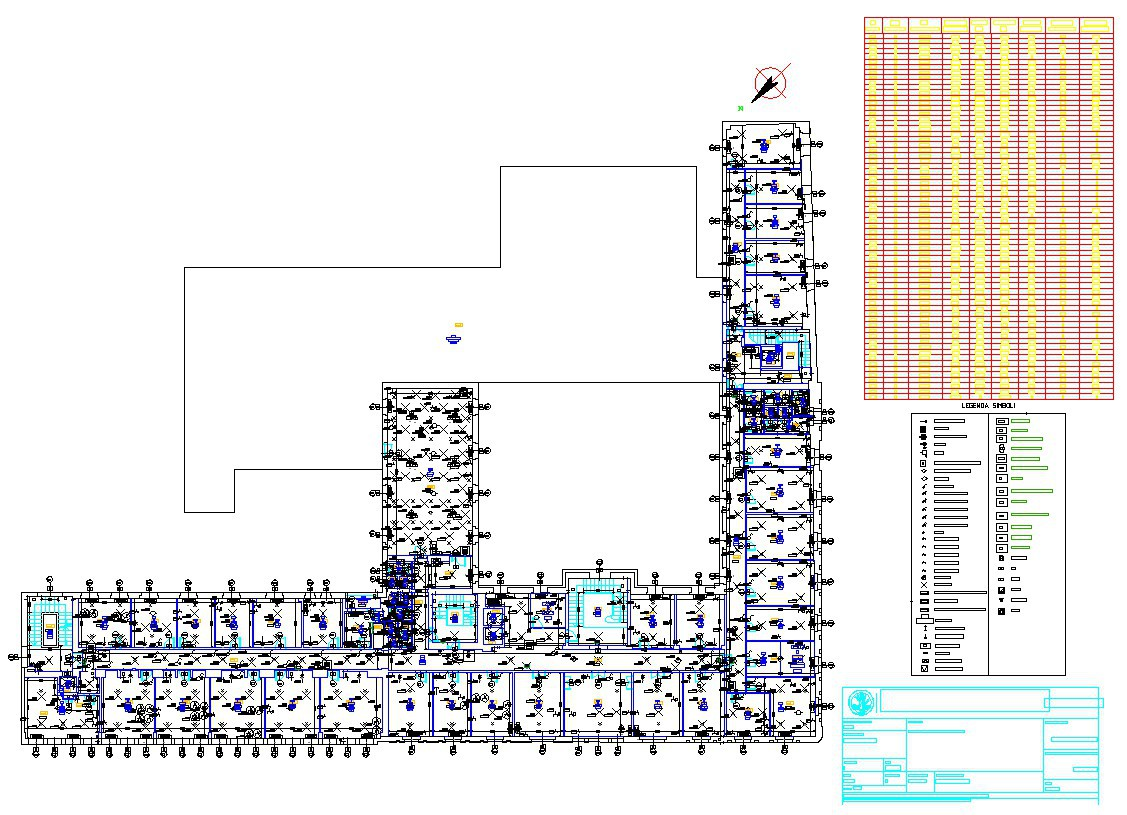
\includegraphics[width=\textwidth,natwidth=1127,natheight=815]{03-dxf-chaos.jpg}
    \caption{Esempio del contenuto di un file DWG di media complessità
(Dipartimento di Informatica, 1º piano). La quantità di informazioni
presente rende difficile la comprensione del contenuto informativo
del file manualmente. }
    \label{fig:dxf_chaos}
\end{figure}

Con l'aiuto anche della Divisione Sistemi Informativi, rappresentata
da Vincenzo Pupillo, abbiamo ottenuto invece in formato testuale CSV le
informazioni utilizzate dal sistema Easyrooms, rispetto all'uso didattico
degli spazi (eventi, lezioni, capienza delle aule, lauree, eccetera).

Entrambe le divisioni ci hanno aiutato con totale disponibilità e
trasparenza, e senza il loro aiuto il nostro progetto non sarebbe mai
stato portato a buon fine.

Con queste informazioni in mano abbiamo incominciato l'analisi,
cercando di capire non solo le loro criticità, ma anche dove si
sovrapponevano, completavano o fossero ridondanti. Al primo contatto
ci sembravano perfette: avevamo informazioni di destinazione delle
stanze, la loro capienza, accessibilità a disabili, e le potevamo
localizzare sulle piante architettoniche utilizzando dei codici
identificativi presenti anche su quelle. Dalle piante ottenevamo anche
la localizzazione di aree di interesse come biblioteche, sale studio, bagni,
spazi di ristorazione, eccetera.

In sostanza, il lavoro di integrazione consisteva nel far confluire in
prima istanza i dati testuali delle divisioni Sistemi Informativi
e Edilizia. Si trattava allora di relazionare informazioni sui palazzi
e sulle aule didattiche. Il risultato di questa operazione andava 
poi correlato con le informazioni presenti nelle piantine edili. Lo scopo
finale è quello di avere un ulteriore set di dati disponibile, con la
pretesa di essere più preciso e di avere più informazioni delle
singole sorgenti di partenza.

\section{La consistenza dei dati}

A uno sguardo più attento, però, l'immagine mentale che ci eravamo
costruiti di quei dati incominciò a rivelare i suoi difetti: errori di battitura, 
utilizzo di diversi
codici identificativi per i palazzi, piante architettoniche fuori
scala o semplicemente disegno della stessa stanza più di una volta
sullo stesso file. Spesso i disegni venivano ripetuti sulla stessa
posizione, probabilmente frutto di un'operazione di copia e incolla
interrotta a metà. Gli errori saltavano all'occhio facilmente, e
riuscivamo a correggerli riconoscendo dei pattern di riferimento, ma per un
elaboratore non sarebbe stato così facile. Dato che il nostro scopo era 
quello di estrarre le informazioni in modo automatico, 
è stato necessario gestire tutte queste eccezioni/errori.

Con buona probabilità questi errori sono stati accumulati lungo gli
anni, ed è totalmente comprensibile che ci siano, se  consideriamo ad
esempio che la maggior parte delle piante architettoniche di cui
disponevano sono state disegnate in formato cartaceo e solo a posteriori
trasferite in formato digitale, quando la costruzione dell'edificio era già
finita. %%PROF: in che senso? cosa interessa quando sono stati costruiti?
Sono inoltre state fatte e raccolte lungo periodi significativi,
create da persone diverse, e perciò è difficile mantenere degli
\textit{standard} nella loro rappresentazione digitale. Ovviamente, nel
processo di trasferimento da cartaceo a digitale, dettagli vengono persi,
errori vengono introdotti, e le versioni digitali non passano per la stessa
meticolosa verifica di quelle utilizzate per la costruzione degli edifici. 

Da questo segue una nuova sfida: prima ancora di procedere all'integrazione,
dovrebbe esserci un efficace meccanismo di validazione dei dati di partenza.
Questo è diventato un valore aggiunto dell'applicazione, cioè la capacità di
fornire un'analisi della correttezza sintattica/semantica dei file in input, permettendo
un valido \textit{feedback} per ulteriori miglioramenti e correzioni manuali.

Una volta che abbiamo superato le barriere più significative per l'estrazione 
dei dati e riuscivamo effettivamente ad inserirli nel nostro 
database, abbiamo potuto fare un ulteriore passo rispetto a 
queste validazioni di dati: avendo altre fonti con cui comparare i dati
estratti, le operazioni di validazione acquisivano anche un significato
semantico. 
%% secondo me il significato semantico c'era anche prima, ora si aggiunge quello di coerenza/consistenza
%% SAM: hai ragione. troverò con calma un modo migliore per dire
%% quello che intendevo

Infatti, alla fine del progetto abbiamo sviluppato in parallelo
un altro programma in grado di analizzare lo stato del database 
e fornire un lungo e comprensivo \textit{output} sulla 
qualità e quantità dei dati, e sui risultati dell'integrazione delle 
diverse sorgenti. Questo programma ci ha fornito anche delle medie campionarie che ci hanno 
garantito un maggiore livello di confidenza nello scegliere le
strategie per l'estrazione o l'ulteriore elaborazione dei dati.

\section*{Nessuna assunzione}

La mole di dati era significativa, in particolare per i file DXF: più di
700, ognuno con dimensione media di 4.5Mb, e casi estremi anche di
44Mb. Questi file contenevano tutte le informazioni edili: tubature,
finestre, porte, scale, sezioni dei palazzi, disegno dei muri,
cortili, terrazze, eccetera. Ci è bastato poco tempo nell'analizzare quei
dati per capire che l'unico modo di giudicarne la loro qualità sarebbe
stato incominciando con la loro estrazione e imparando durante il
processo. Queste caratteristiche hanno determinato tanti aspetti dello
sviluppo, e in particolate del nostro \textit{workflow}, che frequentemente si è
dimostrato ``REPL \textit{Driven}'' o ``\textit{Experimentation
Driven}''\footnote{Più dettagli nel capitolo \ref{cap:scelta_di_workflow}}. 

Da queste analisi abbiamo concluso che potevamo fare poche o nessuna
assunzione iniziale sulla qualità, formato, presenza o consistenza dei dati.

\section{Le scelte tecnologiche a partire dai dati}

Questa natura dei dati trasformava tante delle nostre richieste in
\textit{``Wicked Problems''}, problemi la cui comprensione potrebbe
avvenire soltanto durante la loro risoluzione stessa e non è
possibile \textit{a priori}. Questo è stato uno dei primi motivi che
ci ha fatto scegliere Python 3 come linguaggio di riferimento per
l'estrazione e l'elaborazione: la capacità di scrivere velocemente
degli script in grado di estrarre e produrre dettagliate analisi delle
caratteristiche dei dati. 

Oltre a questo aspetto, anche i seguenti punti hanno contribuito
alla scelta di Python:
\begin{itemize}
  \item La presenza delle \textit{list comprehentions}, un potente
strumento per l'esecuzione di operazioni di trasformazione e
filtraggio dei dati, specialmente se associate a funzioni per
l'aggregazione di dati e agli iteratori di Python 3. Possiamo vedere
le \textit{list comprehentions} come un'applicazione più leggibile del
paradigma map-filter-reduce;
  \item L'esistenza di una forte comunità di sviluppatori e entusiasti
per il linguaggio, specialmente in Italia;
  \item L'ampia presenza di librerie di supporto per le attività che
dovevamo eseguire (lettura delle piante, elaborazioni geometriche,
generazione di immagini, ecc);
  \item La positiva sfida rappresentata dal fatto che Python era un linguaggio
  quasi nuovo per tutti i partecipanti al progetto;
  \item La convinzione che la scelta di Python non sarebbe stata limitante per 
  la continuazione del progetto da parte di altri studenti/tesisti, in quanto è
anche un linguaggio insegnato all'università.
\end{itemize}

Per quanto riguarda la scelta del DBMS (\textit{Database Management
System}) è stata l'inconsistenza dei dati a guidare la scelta: le
informazioni presenti sui diversi palazzi non erano omogenee in
termini quantitativi nè qualitativi. Su alcuni edifici disponevamo di
più informazioni topologiche mentre su altri quasi nessuna. Anche le
informazioni inerenti all'edificio stesso (come il suo nome rappresentativo o
scopo d'utilizzo - ad esempio ``Dipartimento di Informatica'') non sempre
erano presenti o valide, e ciò si ripeteva anche sugli altri dati. L'uso di un
DBMS relazionale avrebbe portato a degli \textit{schema} con considerevoli
campi \textit{null} e denormalizzato, due aspetti considerati
\textit{anti-patterns} nella progettazione di \textit{database} relazionali.
Per questi motivi abbiamo scelto un DBMS che seguisse un modello di
memorizzazione \textit{schemaless}. 

Per le note caratteristiche prestazionali, supporto nativo a calcoli
su coordinate geografiche, presenza di forte comunità, documentazione
chiara e completa e la diversità di librerie aggiuntive disponibili,
abbiamo scelto MongoDB come DBMS di riferimento.

\section{Partire da Zero}

Una mia particolare preoccupazione in fase iniziale del progetto, era
quella di garantire la costante e continua ricerca di una buona
progettazione. A parte i vantaggi ovvi per il prodotto finale di un
approccio del genere, avevo lo scopo personale di sanare un mio
\textit{gap} tecnico: sentivo che le mie conoscenze di (buona)
progettazione del Software erano molto spesso di carattere teorico. 
Mi mancava l'assimilazione pratica dei principali concetti e avevo
l'impressione che questo \textit{gap} fosse abbastanza comune tra gli altri
studenti del mio stesso anno. Mi sembra anche ragionevole, dato che il
perfezionamento di questo tipo di abilità avviene in modo più
significativo soltanto attraverso il confronto dello studio teorico con
l'applicazione pratica. Su questo aspetto ho trovato un forte contributo nello
sviluppo di questo progetto.

In precedenza, nella mia carriera professionale e accademica, poche
sono state le opportunità in cui ho potuto pensare al design del
software complessivamente. Prevalentemente applicavo i precetti 
di design a livello \textit{micro}: singolo algoritmo,
singola procedura, al massimo singola classe/modulo. Ma spesso
neanche quello potevo fare, dato che la preoccupazione principale era
quella di sintetizzare un algoritmo funzionante e performante, oppure
di esplorare una determinata tecnica o risolvere un problema pratico in un
determinato orizzonte temporale molto preciso.

In ambito accademico sento che il rilievo maggiore è sempre stato 
dato alla performance e al rispetto di vincoli pratici e in poche
occasioni ci siamo concentrati sulle tecniche per l'organizzazione
più strutturata del software. Ovviamente, questo è un discorso
molto generale e queste caratteristiche sono anche comprensibili data
la quantità di argomenti da esplorare nel poco tempo disponibile
su un corso di studi di una laurea triennale.

Pensare a un sistema più complesso, con più componenti e elementi, 
organizzarli e coordinarli, gestire le loro
dipendenze, garantire un isolamento e disaccoppiamento salutare, non sono
compiti da affrontare sotto gli stretti vincoli temporali che hanno 
caratterizzato la maggior parte della mia esperienza accademica o professionale. 

Per quanto riguarda la mia esperienza professionale, la parte più
significativa ha avuto luogo in ambito di sviluppo web, 
e spesso partivo da qualche
\textit{framework}\footnote{
	La maggior parte della mia carriera come sviluppatore ha avuto luogo
	utilizzando \textit{Ruby on Rails}, un \textit{framework} noto per non
	solo fornire una struttura MVC, ma per essere anche fortemente
	\textit{opinionated}, cioè di avere le \textit{best practices}
	definite e incentivate in modo molto chiaro.
} 
o sistema preesistente, che mi forniva già una struttura base
per il \textit{design} a livello macro, 
di solito con l'utilizzo di pattern strutturali come MVC / MVP.
A me restava più che altro da rispettare le convenzioni fornite dall'ambiente di
sviluppo e assicurarmi di, a livello \textit{micro} (metodi, classi), non
causare troppi danni.

Sul progetto Spazi Unimi non avevamo una struttura simile preesistente, e non
avevamo qualcuno all'interno del \textit{team} che ci mostrasse le
soluzioni migliori. Perciò,  abbiamo avuto spesso discussioni per superare la
sfida della costruzione del software da zero. In questo senso,
mi sento fortunato di aver potuto partecipare a un processo
così intenso, e sono grato per l'opportunità di averlo fatto affianco
ai colleghi Diego Costantino e Paolo Venturi. 

Nei prossimi capitoli vi racconto una piccola parte di tutto questo ricco
processo.

% 
% 
%			CAPITOLO 3
\chapter{La scelta di un \textit{workflow}}
\label{cap:scelta_di_workflow}


\section{Partire con il TDD}

Per incominciare lo sviluppo ci siamo messi l'obbiettivo di utilizzare il
\textit{TDD - Test Driven Development}, un consacrato \textit{workflow} per lo
sviluppo software noto per portare a soluzioni di design più semplici, pulite,
disaccoppiate e testabili, tutte proprietà desiderabili da un software. Dato
che sul TDD esiste già una svariata bibliografia online, lo riassumo in poche
parole: consiste sostanzialmente nello scrivere i test delle nuove
funzionalità prima di implementarle, seguendo un preciso flusso di lavoro
(scrivo il test, lo eseguo e lo vedo fallire, implemento la funzionalità e
rieseguo il test fino a farlo passare, faccio \textit{refactoring} e
ricomincio l'iterazione con la prossima funzionalità). 
In questo modo è permesso allo
sviluppatore testare l'interfaccia stessa delle funzioni, metodi, moduli o
oggetti che dovrà sviluppare, per poi andare a riempire i dettagli.

Con questo obbiettivo in mente abbiamo incominciato il progetto
affrontando quello che ci sembrava l'aspetto più difficile e che allo
stesso tempo più ci interessava, cioè l'estrazione dei dati delle
piante architettoniche. Dovevamo allora scoprire in che modo la
libreria dxfgrabber ci poteva aiutare. Naturalmente, abbiamo
aperto la REPL\footnote{
	REPL - \textit{Read Eval Print Loop}. Si tratta di un ambiente di
	programmazione interattivo che ci permette di inserire comandi del
	rispettivo linguaggio di programmazione ed avere il risultato
	stampato in sequenza. 
} 
di Python, e abbiamo incominciato a sperimentare con la libreria e i dati.

La libreria dxfgrabber gestiva il compito di leggere i file da disco,
interpretare le sue informazioni e restituirci un oggetto che
rappresentasse il suo contenuto. Ci forniva la lista di entità
grafiche/geometriche (linee, segmenti, cerchi, raggruppamenti di
oggetti) e i testi, o etichette, tutto rispettando i 
\textit{layers}\footnote{
	I \textit{layers} sono strati diversi su cui gli elementi del file
	vengono collocati. Servono a raggruppare elementi diversi per scopo
	funzionale o semantico, come nell'esempio citato per le porte.
}
con cui il file veniva organizzato. 

La grande maggioranza di questi
file sembrava seguire uno standard preciso per il \textit{naming} dei
\textit{layers}: c'era un \textit{layer} ``PORTE'', un \textit{layer} 
``RM\$'' che conteneva i poligoni delle stanze, un \textit{layer}
``FINESTRE'', e così via. Ma in qualche file, Il \textit{layer} ``PORTE''
potrebbe chiamarsi ``PORTA'', le finestre potrebbero essere state
inserite insieme alle murature nel \textit{layer} ``MURI'', mentre
il \textit{layer} ``SCALE'' era vuoto con le scale disegnate
insieme alle stanze su ``RM\$''. Sul \textit{layer} delle porte,
a volte trovavamo le porte disegnate come linee e archi sparsi,
a volte raggruppate all'interno di oggetti composti (chiamati
\textit{Insert}, una specie di gruppo di oggetti), e lo stesso 
valeva per le finestre e le scale. 

\section{Diffidare del TDD}

Avevamo una grossa mole di dati, ma quanto più li esploravamo più
eccezioni trovavamo per le regole che pensavamo aver 
identificato. A questo punto, abbiamo incominciato a chiederci se
il TDD sarebbe stato adeguato per la natura dei problemi che
dovevamo affrontare.

Una delle difficoltà pratiche del TDD è riuscire a convincere un eventuale
\textit{manager} orientato ai risultati immediati che ne valga la pena. 
Il motivo è semplice: all'inizio il TDD tende a rallentare 
il processo di sviluppo. 
%% soprattutto se gli sviluppatori non ne sono esperti
%% Sam: Sono assolutamente d'accordo. Conviene dichiararlo nella tesi però? 
%% Ho cercato di trovare un punto di equilibro che mi permettesse parlare
%% degli errori che abbiamo commesso ma con più attenzione a come li abbiamo
%% superato.
I suoi benefici si evidenziano successivamente, 
sotto forma di un \textit{design} del software più consistente,
manutenibile, semplice, e chiaro. Spesso i test scritti per guidare 
la progettazione aggiungono anche valore ulteriore 
come \textit{regression test}. Riassumendo, 
il TDD ha un costo immediato, ma tende a ripagare a lungo
termine in forma di un \textit{design} di qualità superiore, e questo
sembra abbastanza evidente per la maggior parte degli sviluppatori.

È noto in ambito informatico il fenomeno caratterizzato
dalla difesa quasi religiosa delle tecnologie utilizzate da un
particolare gruppo di sviluppatori. Lo stesso ho potuto
osservare rispetto al TDD con determinata regolarità e intensità.
Uno sviluppatore che si dichiari
sfavorevole al TDD, che affermi di non utilizzarlo tutto il tempo o 
nella sua forma più tradizionale deve prepararsi a venir 
contraddetto in poco tempo\footnote{
	Giusto per citarne un esempio,
	uno di questi episodi ha (per fortuna!)
	portato a una epica discussione\cite{fowler_tdd_dead} fra David Heinemeier Hansson (che ha dato inizio alla discussione\cite{dhh_tdd_dead}),
	Martin Fowler e Kent Beck.
}.
	
Ovviamente queste sono mie particolari osservazioni senza nessuna
pretesa di valore scientifico. Il mio obbiettivo nel
richiamare questo aspetto è quello di discutere su possibili
contesti in cui i benefici di utilizzare il TDD possono non bilanciare
in tempo  i suoi costi. 

Nel nostro caso, l'eterogeneità dei dati da trattare rappresentava 
una notevole sfida per la scrittura dei test. Una delle qualità 
del TDD sta nel fatto che molto spesso, quando non si sa 
come incominciare a implementare una funzionalità, si è in
grado di scrivere almeno i test che andranno a testarla. Nel nostro
caso, la difficoltà di fare assunzioni su come i dati di input 
si dovrebbero presentare faceva si che nessun test scritto 
ci sembrasse ragionevole. I nostri tentativi generavano casi di 
test che si basavano su assunzioni che non eravamo in grado di 
dimostrare. Le poche che abbiamo provato si sono rilevate composte 
più da eccezioni che da regole.

Per poter procedere con l'utilizzo del TDD come guida dello sviluppo,
abbiamo capito che, ad ogni iterazione, avremmo potuto
procedere in uno di questi modi:

\begin{itemize}
  \item Basandoci sui file veri. Usando molti file avremo suite di test
  eccessivamente lente (I/O di file di dimensione significativa),
  usandone pochi avremo affidabilità insufficiente. 
  \item Basandoci sull'uso di \textit{mock} 
  per poter stimolare una quantità significativa di casi, 
  senza dover pagare gli eccessivi tempi di I/O dei file veri. 
  La difficoltà stava nell'elaborazione dei casi di test: o 
  sarebbero stati casi fittizi e di conseguenza non avremmo potuto giudicarne 
  l'affidabilità, oppure avremmo dovuto esplorare i file veri in modo
  sistematico per poter ottenere riferimenti di casi veri da trattare.
\end{itemize}

In entrambi i casi i vantaggi del TDD diminuivano di fronte al costo della
scrittura dei casi di test. Testare la prima estrazione
avrebbe richiesto uno sforzo molto alto perché eravamo
circondati da incertezze.
%%PROF: nota per il futuro: in questi casi (incertezza sul da farsi o poca conoscenza di framework, o librerie che si devono usare) il modo di procedere è quello di fare uno spike esplorativo (quello che voi avete fatto tramite REPL), ma poi una volta eliminata un po' di incertezza, si passa al TDD :-D 
%% SAM: Abbiamo sbagliato parecchio durante il progetto. Questo è sicuramente
%% uno dei punti più significativi. Grazie prof :)

\section{Accogliere l'incertezza}

Analizzando le opzioni, l'unica possibilità era cercare di
trattare l'incertezza. Avevamo bisogno di fare qualche assunzione, ma
non riuscivamo a trovare proprietà che venissero rispettate nel 100\%
dei casi. La via di uscita sarebbe dimenticarci dell'ideale 100\%.
Non l'avremmo mai raggiunto. Ci serviva, invece, una soglia ammissibile di
errore, la possibilità di segnalarli all'utente o superarli attraverso qualche
euristica particolare. Identificammo allora i seguenti obbiettivi, per ogni
funzionalità / problema in considerazione: 

\begin{itemize}
  \item Definire la soglia di errore ammissibile.
  \item Superare la maggior parte possibile di errori, con uso di
euristiche diverse selezionate in modo il più complementare possibile.
  \item Rilevare errori non risolubili per rendere possibile
all'utente la loro correzione manuale. In questo modo, anche se non
riuscivamo a soddisfare la soglia di errore ammissibile, avremmo
sviluppato un sistema in grado di riconoscere le proprie limitazioni.
\end{itemize}

In altre parole, non saremmo più partiti dai test, ma da un'esplorazione
sistematica del problema e dei dati, e infatti era esattamente quello che
avevamo già fatto alla prima apertura della REPL per l'esplorazione della
libreria utilizzata: volevamo capire meglio in che modo lo strumento ci
potesse aiutare nella gestione dei dati. Tale approccio ci ha consentito di
gestire meglio l'incertezza, sostituendo le assunzioni per ipotesi da testare.

In uno \textit{speech} nell'Agile UX NYC 2012, Joshua Seiden discorre
sul rimpiazzare i \textit{requirements} con ipotesi quando sviluppiamo
per ambienti caratterizzati dall'incertezza: 

\begin{quote}
Quando si è in produzione, sviluppando su standard predefiniti, si vogliono
i requisiti. Quando si è in un ambiente di incertezza, si vogliono
ipotesi.\cite{seiden2012}

\flushright
\textit{(Traduzione mia, originale in inglese\footnote{
``When you're in production, building to known standard, you want requirements. 
When you're in an environment of uncertainty, you want hypotheses.''
})
}
\end{quote}

L'autore sottolinea che molto spesso i \textit{requirements}
nascondono forti assunzioni sugli effetti dei cambiamenti, e la
tecnica suggerita di esprimerli in forma di ipotesi è utile nell'esplicitare
l'incertezza. Abbiamo adottato un approccio simile nel gestire le assunzioni
che facevamo sui nostri dati, attraverso la definizione di soglie di errore
come delle ipotesi di soddisfacibilità dei nostri requisiti.

In seguito allo stabilire delle ipotesi sui dati, seguiva la fase
della loro validazione, dalla quale volevamo ricavare la percentuale
di soddisfacibilità (cioè quale percentuale dei dati totali soddisfa
positivamente o negativamente l'ipotesi in questione).

%%PROF: arrivato qui a correggere
\section{\textit{Experimentation Driven}}

Dalla necessità di conoscere meglio il dominio dei nostri dati e
di testare le nostre ipotesi siamo stati portati a un ciclo di sviluppo
che ho chiamato \textit{Experimentation Driven Development}. 
Si noti che il suo scopo non è il \textit{design} del software,
e che questo modo di procedere non si oppone all'uso del TDD, ad esempio. 

Per \textit{Experimentation Driven Development} intendo una modalità
pratica di sviluppo del \textit{software} che attraverso l'esplorazione
pratica del dominio applicativo, dei problemi da risolvere, e della natura dei
dati, si prefigge di:

\begin{enumerate}
	\item Garantire una comprensione più approfondita del problema.
	\item Capire caratteristiche importanti/comuni su una mole
considerevole di dati.
  \item Rivelare in che modo il linguaggio utilizzato, i suoi moduli o
librerie esterne possono contribuire alla risoluzione del problema
  \item Confrontare ipotetiche soluzioni con grandi quantità di input
non fittizi per capirne la precisione e/o \textit{recall}.
	\item Permettere una naturale validazione e conseguente migrazione
degli approcci di esplorazione utilizzati verso un'implementazione funzionante.
\end{enumerate}

È imprescindibile che l'esplorazione avvenga nell'ambiente stesso su
cui avverrà l'implementazione. Per questo motivo abbiamo utilizzato la
REPL, con l'interprete python bpython\footnote{
\url{http://www.bpython-interpreter.org/}}, che fornisce diverse
 funzionalità utili per un approccio del genere:

\begin{itemize}
  \item Colorazione del codice per facilitarne la comprensione
  \item \textit{Indenting} automatico, il che risparmia considerevole
tempo scrivendo codice su Python, in cui l'indentazione è significativa.
  \item Introspezione sui metodi e funzioni utilizzate, esibendo
direttamente sulla REPL dettagli sulla loro \textit{signature} e anche
documentazione (\textit{docstring}).
  \item Possibilità di salvare il codice utilizzato direttamente
sul \textit{filesystem}
  \item Funzionalità \textit{rewind}, che permette di annullare le
istruzioni eseguite, tornando agli stati precedenti dell'esecuzione. Ci permetteva ad esempio di esplorare e
trasformare i dati per vederne determinati risultati, tornare indietro 
e riprovare con strategie diverse.
\end{itemize}

Infatti è considerevolmente più difficile l'esecuzione di questo approccio
senza tecnologie che riducano i ritardi all'ottenimento
di \textit{feedback}, come ad esempio tempi di compilazione eccessivi.
Il nostro \textit{workflow} basico era composto dai seguenti passi,
eseguiti in modo iterativo:

\begin{itemize}
	\item Comprendere teoricamente la natura del problema
	\item Utilizzare la REPL per conoscere meglio i dati e le sfide
implementative, analizzando la numerosità totale degli input e la
quantità di casi che soddisfano qualche insieme di proprietà desiderate.
	\item Creare/salvare codice che permetta o la risoluzione del
problema (in termini di soglie ammissibili) o l'esecuzione di test
significativi sulle funzionalità da implementare.
\end{itemize}

Ad ogni iterazione, le prove precedenti e codici ottenuti venivano
riutilizzati e permettevano una più ampia comprensione, oltre a
generare dei prototipi/bozze implementativi.

Il prototipo/bozza differisce da una versione finale a volte per
aspetti di completezza (può non gestire ad esempio casi limite), a
volte per qualità del codice o prestazioni (viene scritto il più
veloce possibile in modo da non bloccare il \textit{workflow}, ma non
necessariamente si tratta di un'implementazione efficace o chiara).

Non abbiamo scelto esplicitamente nessuna di queste metodologie di
lavoro, piuttosto ci siamo fatti guidare dalla natura dei problemi e
dei dati da trattare. 

\section{La risoluzione dei problemi come conseguenza della loro comprensione}

Uno dei principali obbiettivi del nostro progetto era l'integrazione
semantica delle piante architettoniche. Ciò significa che oltre ad
essere in grado di ottenere il disegno dei piani, volevamo
identificare le stanze in modo da poter fornire informazioni sulla loro
destinazione d'uso. 

Era un nostro interesse essere in grado di dire a un utente
dove si trovasse la specifica Aula/stanza del suo interesse all'interno
di un palazzo, oppure informare la localizzazione di stanze a seconda
della categoria di cui l'utente avesse bisogno. In altre parole, 
associare alla pianta architettonica
stanze specifiche (esempi: ``Aula Beta'', ``Aula 206'', ``Stanza P116'')
oppure riconoscere le loro categorie, tipologie o 
destinazione (esempi: Bagni, Ascensori, Sale Lauree, Sale Informatiche,
Biblioteche, ecc).

L'ottenimento del formato (disegno) delle stanze è stato poco 
problematico. Abbiamo incominciato l'esplorazione 
con l'unico obbiettivo di comprendere meglio i dati e
il problema, e di conseguenza abbiamo prodotto la soluzione.
Partendo sempre dalla REPL siamo riusciti a 
ottenere, a piccoli passi, i codici per portare avanti quelle
estrazioni. 

A mio modo di vedere partire con il TDD in questo caso avrebbe 
rallentato significativamente lo sviluppo iniziale. Da un altro lato,
abbiamo sentito posteriormente la mancanza di un approccio sistematico 
per quanto riguarda il design, e su questo argomento ritorneremo più
in avanti.

Abbiamo elaborato i test posteriormente, per aumentare la confidenza 
ad ogni risultato raggiunto e permetterci di proseguire con 
l'esplorazione senza rischiare di invalidare le conquiste precedenti.

\section{Prendere decisioni dalla REPL: un esempio pratico}

Le difficoltà tecniche maggiori sono sorte nell'associare le etichette alle
relative stanze. L'unico vincolo fra le etichette di una stanza e il
suo disegno era la loro relativa posizione, senza altre indicazioni a
livello sintattico. Abbiamo allora utilizzato un algoritmo che, dato
un poligono S (stanza) e un punto P nello stesso spazio di riferimento
(punto di ancoraggio dell'etichetta testuale), rispondeva 
alla domanda ``Il punto P è dentro il poligono S?''.
Si tratta di un algoritmo particolarmente
interessante e concettualmente semplice, chiamato \textit{Ray Casting
Algorithm}\footnote{Una chiara spiegazione è presente su Wikipedia:
\url{http://en.wikipedia.org/wiki/Point_in_polygon\#Ray_casting_algorithm}}.

La nostra ipotesi sui dati era che, essendo in grado di rispondere a
questa domanda, saremmo riusciti ad associare etichette correttamente
al 90\% delle stanze\footnote{La scelta di questa soglia era
giustificata dal fatto che in mezzo ai file di cui disponevamo c'erano
anche altri file che non ci davano informazioni utili, o che si
riferivano a palazzi non utilizzati per scopi didattici, in cui la
percentuale di identificazione di stanze sarebbe naturalmente più bassa}.

In presenza di stanze piccole o strette (come corridoi ad esempio),
poteva capitare che l'etichetta, per mancanza di spazio, venisse
collocata all'interno di una stanza vicina. All'occhio umano era
semplice capire a quale stanza tale etichetta appartenesse, ma un po'
più complicato in termini algoritmici.

\begin{figure}[H]
    \centering
    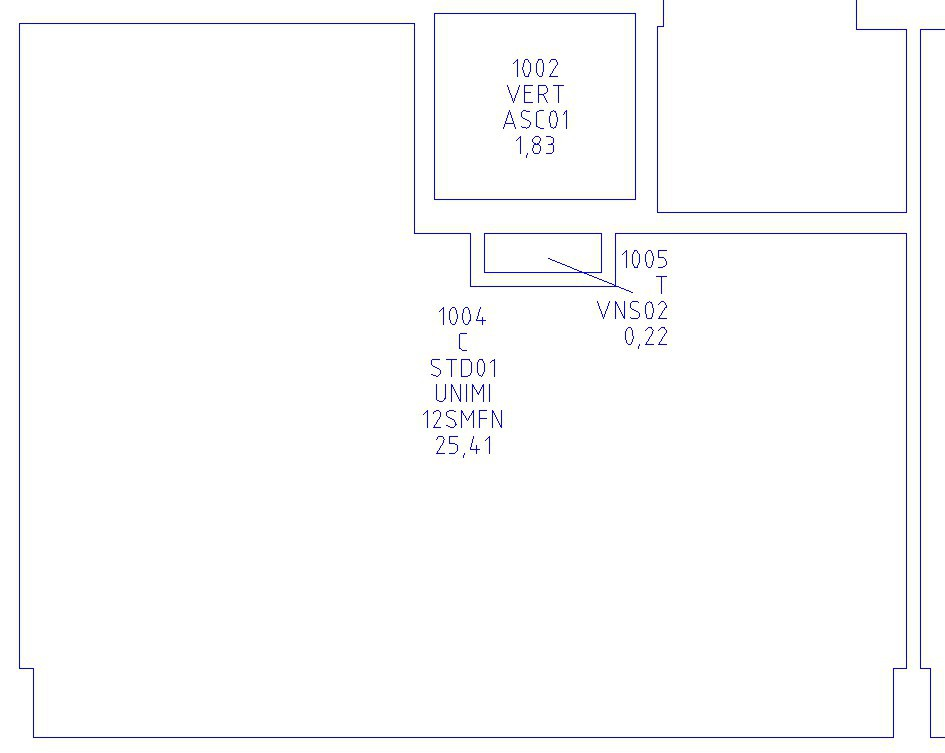
\includegraphics[width=300pt,natwidth=945,natheight=753]{03-dxf-stanza-etichette-fuori.jpg}
    \caption{Esempio di stanza con più etichette al suo interno. L'etichetta 
    corretta è quella indicata dal numero 1004. Quella di numero 1005 è
    riferita al piccolo rettangolo indicato (in questo particolare caso,
    ma non sempre è così) dalla linea uscente, e si tratta di
	un ``Cavedio Porta Impianti'', cioè uno spazio per il passaggio dei cavi.
	}
    \label{fig:dxf_room_labels}
\end{figure}

Avevamo stabilito l'ipotesi d'interesse e dovevamo allora testarla.
Utilizzando la REPL, abbiamo analizzato tutti i file e ottenuto
la quantità esatta di stanze con etichette associate. Sul totale di
stanze rappresentava circa il 96\%, e questo ci ha fatto intuire che
la nostra ipotesi poteva effettivamente essere verificata.
Avevamo in mano, dall'uso della REPL, una soluzione che sembrava 
soddisfacente. Non eravamo sicuri di avere il 90\% di \textit{precision}
desiderato ma sembrava abbastanza vicino. Restava allora da stimare
la correttezza.

Purtroppo definire la correttezza sarebbe stato un lavoro manuale. Facendolo,
ci sembrava ancora ragionevole la nostra ipotesi. Abbiamo identificato errori,
ma in media erano pochi. Era però un lavoro molto lento.

Per evitare di dover analizzare più di 700 file manualmente,
abbiamo allora lanciato una nuova ipotesi: se scartiamo alcune
tipologie specifiche di stanze che ai nostri scopi sono di minore
importanza, riusciremo ad aumentare la precisione relativa al 90\%
desiderato, a patto di ridurre il percentuale di \textit{recall}.

Nell'esempio sopra il nostro algoritmo poteva sbagliare o decidere 
correttamente con uguale probabilità: dipendeva soltanto da quale 
delle due etichette venisse considerata prima in confronto al 
poligono della stanza. Decidendo di non considerare l'etichetta 
1005 per il fatto che si tratta di un ``cavedio porta impianti'' 
(codice VNS02 associato) l'unica possibilità sarebbe stata
la risposta corretta. Avevamo identificato tanti altri casi simili, e
ci aspettavamo che ce ne fossero altri.

La scelta di queste categorie non partiva solo dal fatto che a noi
interessavano meno. Abbiamo cercato di sceglierle
in modo intelligente. Il problema delle etichette si verificava
quando stanze molto piccole o strette erano presenti,
perché era quello il motivo per cui le etichette finivano all'interno del
poligono di un'altra stanza, come nell'esempio sopra 
del ``cavedio porta impianti''.

Tra le categorie che avevamo selezionato da scartare c'erano anche 
gli ascensori, i bagni e le scale.
Tra tutte queste, però, solo il ``cavedio'' sembrava effettivamente
trascurabile ai nostri scopi.

Con l'uso della REPL abbiamo eseguito delle prove veloci manipolando i
codici già esistenti in modo che scartassero soltanto le etichette di
tipo ``cavedio'', con lo scopo di misurarne gli effetti.
Il risultato è stato positivo: c'è stato un
trascurabile calo nel tasso di \textit{recall} (infatti pochissimi casi
di cavedio avevano l'etichetta posizionata correttamente all'interno del
piccolo poligono relativo), e un aumentare del percentuale di stanze
di altre categorie più rilevanti che prima venivano associate 
all'etichetta sbagliata.

In un momento successivo ci siamo accorti che non dovevamo necessariamente
scartare altre categorie, come corridoi o ascensori. Ci bastava definire un
ordine di priorità: analizzare tutte le stanze e cercare di associare solo
le etichette note per indicare locali di dimensione ragionevole (aule, aule
informatiche, sale lauree, sale studio, biblioteche, ecc), e solo in un 
secondo momento cercare di associare le categorie di locali più piccoli ai
poligoni non ancora associati. L'ipotesi era semplice: la probabilità
che le categorie della prima analisi generassero errori
era molto più piccola, assumendo che il posizionamento delle etichette
era stato fatto da esseri umani, e che allora per stanze di dimensione
significativa dovrebbero essere collocate al loro interno.

Con l'uso della REPL abbiamo invece scoperto che tale approccio non era
necessario: la differenza nella qualità dell'associazione era molto
bassa. Da ciò abbiamo concluso che la soluzione precedente, con grande
probabilità, soddisfaceva già la nostra precisione desiderata del 90\%.
Non era giustificata allora la complessità aggiunta in termine di 
codice, e allora abbiamo mantenuto soltanto lo scarto della 
categoria ``Cavedio porta impianti''.

Questo è un esempio di una metodologia che abbiamo utilizzato più volte, in
speciale nell'affrontare l'estrazione e comprensione dei dati originati
dalle piantine architettoniche.
Sono casi in cui l'uso della REPL per l'esplorazione prima
dell'effettiva scelta degli algoritmi ci ha permesso
di affrontare i problemi in modo più efficiente e con più
sicurezza. Ci permetteva velocemente di capire caratteristiche comuni
o analizzare attributi dei dati per provare alternative, e poi migrare
quelle conclusioni verso un'implementazione effettiva. Creando
ipotesi, dimostrando che coprissero i casi prevalenti e aggiungendo in
seguito euristiche per l'inclusione di più casi specifici, siamo riusciti ad
affrontare la maggior parte delle difficoltà.

A volte ottenevamo dalla REPL un modulo già semilavorato, a volte
semplicemente una media campionaria che ci permetteva di avere più
confidenza nelle scelte prese.
Quando una precisione assoluta e deterministica non era possibile,
l'analisi delle qualità dei dati giustificava assunzioni che ci
permettevano di procedere a un'estrazione \textbf{sufficientemente o
statisticamente buona}, superando la difficoltà di correggere errori
umani. In altre parole, ci permetteva di continuare anche quando in
termini assoluti sarebbe stato sbagliato farlo.

L'ultimo vantaggio di questa metodologia è quello di garantire un
rapido \textit{feedback} per le strategie adottate. Di certo non tanto
rapido e riproducibile quanto una suite di test, 
ma nel contesto in cui la scrittura
dei test sarebbe stata problematica, l'uso della REPL ha agevolato
significativamente la valutazione manuale e l'ottenimento di statistiche.

Vale notare che è un approccio iterativo e incrementale. Si cerca di partire
dalle ipotesi che giudichiamo porteranno ai migliori risultati immediati
e di aggiungere successive ipotesi che considerino casi complementari. Si 
ferma quando la precisione raggiunta viene giudicata sufficiente.

\section{Il problema dell'integrazione dei piani}

Un altro momento in cui l'analisi statistica dei dati e dei file è
stata essenziale è stato durante la fase di integrazione di informazioni sulle
stanze e piani di ogni edificio. Alla fine della fase di ottenimento dei
dati da tutte le sorgenti, abbiamo scoperto che non esisteva nessun 
standard identificativo per i piani che venisse rispettato da tutte. 
Non c'era un modo diretto per, dati due piani di due sorgenti diverse,
stabilire se si riferivano allo stesso piano fisico. Ciò rendeva 
l'integrazione dell'informazione sulle stanze molto difficile.

I dati ottenuti dall'Edilizia identificavano i piani con lettere e numeri, 
(t, 1p, 2p, ecc) a seconda del caso, ma non era una convenzione unica 
e potevano esserci più identificativi per uno stesso tipo di piano. 
Easyroom, invece, utilizzava una convenzione molto precisa, 
basata su numeri interi: i negativi indicavano piani sotterranei,
lo zero il piano terra e poi in sequenza gli altri piani (1, 2, ...). 

La soluzione più intuitiva sarebbe quella di utilizzare una mappatura fra
queste diverse convenzioni di identificativi. Però, esplorando
i dati sulla REPL abbiamo scoperto casi particolari che impedivano un
approccio del genere. Esistevano palazzi la cui struttura di piani
secondo il dip. di Edilizia era di questo tipo:

\begin{itemize}
	\item 1º Sotterraneo
	\item Terra
	\item Ammezzato
	\item 1º Piano
	\item 2º Piano
\end{itemize}

Al posto di Ammezzato ci potrebbe essere Rialzato. In molti casi
il piano Terra non era presente e invece c'erano sia Rialzato che
Ammezzato. Queste distinzioni sono naturali in ambito edile, ma poco
intuitive per l'utente normale di un sistema come Easyroom. Per questo 
motivo, Easyroom collassava le stanze di tutti i piani ``simili'',
come Terra, Ammezzato e Rialzato in un solo piano, di solito quello
più intuitivo (Terra). Abbiamo verificato casi in cui le stanze del piano 
sotterraneo vengono dichiarate insieme a quelle del piano Terra.

Inoltre abbiamo scoperto che gli identificativi dei piani di ciascuna sorgente
erano caratterizzati da un ulteriore incertezza. La seguente 
tabella di esempio (non esaustiva) riassume un po' la difficoltà:

\vspace{1cm}
\begin{tabular}{ l c r }
  \hline
  \textbf{Piano}              & \textbf{Edilizia} & \textbf{Easyroom}    \\
  Sotterraneo / 1º Interrato  & s2 / ip / 1ip     & -1                   \\
  Seminterrato                & sa / s1 / sp      & Non considera        \\
  Terra                       & t / tp / ra       & 0                    \\
  Rialzato                    & ra / rap          & Non considera        \\
  Ammezzato                   & ap                & Non considera        \\
  Ammezzato Rialzato          & arp               & Non considera        \\
  Primo                       & 1 / 1p / p1 / 1ap & 1                    \\
  Secondo                     & 2p / 2 / 2ap      & 2                    \\
  \hline
\end{tabular}
\vspace{1cm}

Considerando allora la pluralità e ambiguità di casi possibili,
il fatto che spesso i file delle piante venivano pure identificati 
con i codici sbagliati (ad esempio con il codice tp,
ma che si trattavano in realtà del 1º piano e non del piano terra), 
e il fatto che Easyroom facesse collassare stanze di piani 
\textbf{diversi} sotto lo stesso identificativo, abbiamo dovuto 
procedere un'altra volta con un approccio basato sulle ipotesi.

Neanche l'identificazione delle stesse stanze su due sorgenti diverse
era un'informazione sufficientemente affidabile per stabilire l'equivalenza
dei loro rispettivi piani. C'erano \textbf{molti} casi in cui ciò 
avrebbe generato errore. L'unica cosa che potevamo affermare effettivamente
era che le piante architettoniche ci garantivamo almeno un raggruppamento
corretto di stanze. Se poi si trattava del piano 0, 1, 2 o sotterraneo
era un altro discorso.

Partendo da questa ipotesi, abbiamo cercato di rimappare non i piani, ma 
le stanze delle due sorgenti \textbf{verso le piante architettoniche}.
La REPL ci ha permesso di stabilire che su un impressionante
99\% dei piani era possibile trovare almeno una stanza, utilizzando il
suo codice identificativo, che venisse rintracciata in tutte e tre le
sorgenti (piantine, informazioni testuali dell'Edilizia e informazioni
testuali di Easyroom). 

La presenza di quella stanza ci dava un'informazione ortogonale 
alle diverse sorgenti. Sapere in quale piano una stanza veniva rimappata 
su ogni sorgente era una forte indicazione di come quei piani potessero
venir relazionati. Rimanevano i casi estremi, ovvero 
le stanze di piani diversi raggruppate sullo stesso piano da Easyroom. 

È stata la REPL a fornirci la sicurezza che ci ha permesso di
proseguire nell'implementazione dell'algoritmo finale, che gestisce tutti i
casi sopra elencati, ed \textbf{è in grado di capire e gestire} i casi in
cui non è possibile trovare un'associazione soddisfacente fra i piani. 

In questo modo all'utente vengono segnalati i conflitti, sia quelli
che abbiamo risolto in modo automatico che quelli la cui risoluzione
non è possibile. Con l'uso di questa strategia e una serie di
euristiche per renderla più efficiente, siamo stati in grado di
associare il 99\% dei piani correttamente. L'errore che rimane
è costituito da precisamente tre casi, due dei quali si presentano solo a
causa di errore di battitura dei dati originali (stanze identificate in
modo sbagliato), e comunque vengono tutti e tre segnalati per la
revisione dell'utente. 

\section{\textit{Nota sul testare}}

Molti componenti dell'applicazione finale sono nati a partire da
questi esperimenti con la REPL. Come detto in precedenza, 
il principale vantaggio era quello di poter 
conoscere la natura dei problemi o i limiti e le potenzialità 
delle nostre scelte algoritmiche, senza dover pagare un prezzo 
troppo alto se mai fosse necessario tornare in dietro.

Questo \textit{workflow} fece si che nessun componente prototipale
rimanesse intoccato per molto tempo. In conseguenza dell'aggiunta di
nuove funzionalità o di cambiamenti del codice esistente, per ad
esempio gestire più casi, le componenti venivano rielaborate,
ritrasformate. In sostanza, l'estensione di pezzi
preesistenti diventò un punto essenziale del
processo di sviluppo, e per renderlo possibile abbiamo dato più 
importanza ai \textit{regression test} e a una 
modularità e incapsulamento che ci permettessero di 
cambiare il codice con sufficiente confidenza. 

Rimane da dire come è stata superata la difficoltà del \textit{testing}, che
ci aveva fatto rifiutare l'approccio iniziale del TDD. Una volta che avevamo
affrontato la diversità dei dati con l'approccio di esplorazione, avevamo
dimostrato diverse delle nostre ipotesi, e a quel punto eravamo anche in grado
di scrivere dei test che confrontassero il modo in cui il nostro codice si
relazionava con quelle ipotesi. Non dovevamo più testare la funzionalità di
per se (o i requisiti), ma le ipotesi che avevamo definito e che ci fornivano
il margine desiderato. 

Con la costruzione delle \textit{fixtures} necessarie per testare
le ipotesi base, e con l'aggiunta di quelle per le ipotesi complementari,
siamo riusciti ad avere un'adeguata confidenza in termine di 
test funzionali e principalmente di unità. L'esplorazione ci 
ha fornito la comprensione dei
problemi e anche la capacità di testarli.

\section{\textit{Noncontinuous refactoring}: pagando gli interessi}

\vspace{3mm}
\begin{flushright}
\textit{``Experience is simply the name we give our mistakes.'' - Oscar Wilde}
\end{flushright}
\vspace{8mm}

Avere un insieme di test su cui ci fidavamo è stato essenziale per
garantire l'avanzamento dello sviluppo, ma
non era sufficiente per metterci al riparo della perdita del
design a lungo termine. Questo processo di rielaborazione di 
codice per aggiunta di nuove funzionalità ha finito per portare 
il nostro \textit{codebase} a un punto da cui non riuscivamo più a procedere.
Si trattava del noto fenomeno del \textit{Software Decay}, che purtroppo
non avevamo prima anticipato.

Con un approccio incrementale, il costo degli errori sulle scelte
algoritmiche è stato tendenzialmente contenuto, dato che li potevamo
rilevare presto. Lo stesso non succedeva sugli errori del design.

Quando si parla di TDD, si incomincia solitamente dal ``Test first'', 
il suo lemma principale. Spiegando con un po' più di dettaglio, vengono 
introdotti gli altri quattro passi inerenti al TDD: verificare il 
fallimento del test, farlo passare, eseguire il refactoring, e ripetere. 
Non può coesistere l'idea di fare il TDD e di saltare uno 
\textbf{qualsiasi di questi step}, ma intanto molto spesso ci si limita
a riassumerlo sotto il lemma ``Test First''. 

Dalla scrittura iniziale del test si ottiene l'orientamento per il design 
e ovviamente il test stesso, che contribuisce alla verifica della correttezza
e - molto importante - funziona come \textit{regression test}.
Verificare il suo fallimento garantisce che venga effettivamente eseguito, 
e che sia significativo, cioè che ne attesti l'assenza del
comportamento desiderato. Farlo passare, ovviamente verifica
l'aggiunta della funzionalità. 

Tutto ciò avviene allora in modo incrementale e iterativo, inclusa 
l'attività di refactoring. È essenziale che il \textit{refactoring} 
abbia la stessa dignità e importanza di ogni altro passo affinché il 
TDD sia veramente un approccio verso il \textbf{design}, e non verso 
il \textit{testing}. Lo scopo è quello di garantire una manutenzione 
continua della qualità del design. Ciò dovrebbe evitare il suo decadimento
e allora la necessità di interventi dedicati alla sua risistemazione.

Gli esempi forniti fino al momento e la parte del processo raccontata
non riguardano l'argomento del design del software, e neanche il concetto
di ``continuous refactoring'', ma la naturale adozione di un particolare 
\textit{workflow} per lo sviluppo. La natura di questi problemi ci ha 
vietato l'uso sistematico del TDD, e ci ha portato all'adozione naturale 
di altre strategie. 

Non si trattava di design del software, ma di esplorazione per la 
comprensione. A misura che riuscivamo ad avere implementazioni 
soddisfacenti per ogni funzionalità, le incorporavamo al \textit{codebase}
principale e proseguivamo verso l'esplorazione di ulteriori limiti 
e possibilità.

Non potendo partire dai test, avevamo concluso che il TDD non era
l'approccio più adeguato per \textbf{quella fase dello sviluppo}. 
Però, abbiamo dovuto pagare un alto prezzo per non esserci accorti 
che gli altri lemmi del TDD, in particolare quello del refactoring 
continuo, sono ugualmente importanti. Sul nostro approccio incrementale 
basato sulla REPL e sulla sperimentazione sarebbe stata semplice 
l'introduzione del refactoring continuo/iterativo,
ma non l'abbiamo fatto.

Per altre funzionalità, in particolare quelle successive, di integrazione 
dei dati già estratti, siamo stati in grado di applicare il TDD nella 
sua forma più naturale. È notevole la differenza dell'output di 
queste operazioni rispetto a quelle precedenti, che sta, nella 
mia opinione, nella sistematica e continua applicazione del refactoring.

Siamo arrivati al punto in cui la complessità del sistema era 
cresciuta, e capire il suo flusso non era più immediato. Avevamo 
in mano una serie di classi che, non avendo ricevuto lo sforzo 
continuo per il loro contenimento, incominciavano a rappresentare 
difficoltà per le modifiche o aggiunte di nuove funzionalità, 
mentre su altri moduli avevamo significativa confidenza. Nella 
mia opinione la differenza fra questi casi stava necessariamente 
nella presenza o assenza del refactoring continuo.

Dati i tempi stretti, nella maggior parte dei casi abbiamo optato per
la rielaborazione dei prototipi esistenti e non per il loro scarto,
poiché ci sembrava evidente che una nuova versione fatta da zero avrebbe avuto
molto in comune con il prototipo in mano. Riflettendo a posteriori, vedo
in queste decisioni un ulteriore errore: ci siamo negati l'opportunità 
di ripensarli con uno sguardo più fresco, senza i vincoli 
dell'incertezza che avevamo già affrontato. 

% 
%
%
\chapter{Un Primo Contatto con il \textit{Software Decay}}
\label{cap:software_decay}

\vspace{1cm}
\begin{flushright}
	\textit{
	``We cannot solve the problems we have created
	with the same thinking we used in creating them.'' - A. Einstein
	}
\end{flushright}
\vspace{1cm}

Come anticipato alla fine del capitolo precedente, a un certo punto
dello sviluppo mi sono accorto che incominciavamo a fallire. 
Gli algoritmi funzionavano, il programma eseguiva i suoi compiti, ma il
codice diventava intricato e difficile da mantenere.

Non bastava esserci messi l'obbiettivo della ricerca costante della qualità e 
chiarezza del design. Poco a poco, il nostro sistema era diventato complesso, 
le modifiche costavano di più e non potevo evitare di pensare che ci fosse 
qualcosa di sbagliato mentre guardavo il codice, l'organizzazione dei diversi 
moduli, o addirittura la composizione interna di alcuni algoritmi. 

A quanto pare, il nostro progetto, al crescere in dimensione e complessità 
diventava vittima del fenomeno noto come \textit{software decay}.
La nostra desiderata ``buona progettazione'' fatta 
dall'inizio veniva poco a poco storpiata.

L'approccio di sviluppo iniziale basato sulla REPL si era rivelato eccezionale 
per alcuni aspetti, in particolare nella fase iniziale del progetto dove la 
necessità di capire era predominante rispetto alle preoccupazioni sulla 
qualità del codice. Una volta che avevamo superato le limitazioni iniziali dei 
problemi e dati di partenza, il sistema è cresciuto velocemente con l'aggiunta 
delle funzionalità di integrazione dei dati, ulteriori validazioni, interazioni 
con il database e funzionalità di segnalazione. Cresceva in complessità. 

Sentivo ovunque i \textit{code smells}\footnote{
letteralmente ``puzza del codice''}, cioè sintomi sul programma che indicavano 
possibilmente la presenza di problemi più profondi. Tra la percezione dei 
\textit{code smells} e la capacità di trovare le loro radici esiste però una
grossa differenza, e l'esperienza e pratica è ciò che molto spesso ci rende
in grado di stabilire una diagnosi completa.

Mi chiedevo che cosa ci fosse di sbagliato, leggendo il codice e studiando il 
funzionamento del sistema ripetitivamente, senza riuscire però
ad individuare i problemi. Mi mancava. Mi mancava l'esperienza, 
il \textit{know-how} pratico che contraddistingue chi ha già affrontato
queste problematiche: analizzare la propria \textit{codebase} 
ed individuare le cause dei \textit{codesmell}.

Incominciava a dominarmi la paura di modificare il codice, di aggiungere o 
togliere funzionalità. Per compensare mi è venuta l'idea di aggiungere più test
al sistema, per assicurarmi che coprissero la maggior parte di casi possibili.
Con la complessità acquisita, non riuscivamo più a cogliere cosa doveva fare 
ogni pezzo del sistema e come si relazionavano. Una cosa che ci ha aiutato è
stata l'elaborazione di qualche \textit{activity diagram} per almeno rendere 
più esplicito ad altissimo livello i principali flussi di esecuzione 
del programma. 

Ho resistito alla tentazione di aggiungere test per compensare questi difetti,
prima perché mi sembrava sbagliato compensare problemi di \textit{design} (che
addirittura non riuscivo ancora a capire) con l'aggiunta
di test, ma in secondo luogo perché la maggior parte di questi test 
sarebbe stata tautologica, serviva a poco o copriva aspetti già coperti da 
altri. Sentivo ancora che incominciavamo a fallire, una follia.

\section{Tre Programmatori in Cerca di Esperienza}

\begin{quote}
\textit{
(Nota dell'autore: ogni riferimento a scene o persone o drammaturghi italiani
in questo sottotitolo non è puramente casuale)
}
\end{quote}

Non potevo evitare di pensare a quanto mancasse al team un membro più esperto,
qualcuno che avesse già vissuto quella difficoltà e avesse imparato 
da qualcun altro o addirittura a partire da uno sforzo proprio! 
Mi sono accorto però che se qualcuno poteva riuscirci da solo, potevo provare
anch'io, e chi sa un giorno sarei stato io ad aiutare qualcuno in una situazione 
simile? E allo stesso tempo la sensazione di aver bisogno di un maestro che ci mostrasse come procedere era costante.

In mancanza di questa figura all'interno del team, mi chiedevo in che altro modo 
avrei potuto acquisire quell'esperienza. Il primo tentativo 
che considero sia stato un successo parziale è stato quello di 
cercare i concetti teorici della ``buona progettazione'' 
e in particolare sono finito a rileggermi ancora una volta 
i principali materiali disponibili sui principi SOLID\footnote{
SOLID\cite{bobmartin_solid} è un acronimo per i cinque principi basici della programmazione
orientata ad oggetti proposti da Robert C. Martin. I principi sono \textit{
Single
responsibility, Open-closed, Liskov substitution, 
Interface segregation e Dependency inversion.
}
}. 

Dei principi SOLID, l'SRP (\textit{Single Responsibility Principle})
è stato quello più utile, in quanto averlo riletto e applicato alla 
nostra \textit{codebase}, ha comportato 
modifiche significative di tipo strutturale, sia a livello di singolo 
algoritmo che a livello di modulo / classe.

Per capire le responsabilità di ogni classe/metodo, ho utilizzato un
suggerimento di Sandi Metz nel libro ``Practical object-oriented 
design in Ruby: an agile primer'':

\begin{quote}
Un altro modo per concentrarsi su che cosa una classe sta veramente facendo
è provare a descriverla in una sola frase. Ricordarsi che una classe deve
fare soltanto la più piccola cosa utile possibile. Questa cosa dev'essere
semplice da descrivere. Se la descrizione più semplice che si riesce a
ottenere usa la congiunzione ``e'' la classe ha probabilmente più di una
responsabilità. Se utilizza la congiunzione ``o'', allora la classe
possiede più di una responsabilità e non sono nemmeno molto correlate. \cite{metz2013}
\flushright
\textit{(Traduzione mia, originale in inglese\footnote{
``Another way to hone in on what a class is actually doing is to attempt 
to describe it in one sentence. Remember that a class should do 
the smallest possible useful thing. That thing ought to be simple 
to describe. If the simplest description you can devise uses the word ``and,'' 
the class likely has more than one responsibility. If it uses the word ``or,'' 
then the class has more than one responsibility and they aren’t 
even very related.''})
}
\end{quote}

Si noti che secondo Sandi Metz, la presenza di
una unica di queste congiunzioni nella ``frase di responsabilità''
è già sufficiente per concludere che
quella classe ha più di una responsabilità. Pronto, adesso avevo un
principio guida per aiutarmi, a partire dall'analisi sistematica del codice,
a trovare l'origine dei \textit{code smells}.

\section{Esempio pratico di \textit{refactoring} guidato dall'SRP}

Un esempio pratico in cui l'SRP ha contribuito in due granularità diverse è la
classe chiamata DataUpdater, inizialmente responsabile per l'aggiornamento 
delle informazioni sui palazzi e sulle stanze provenienti dalle fonti testuali 
(file CSV). La sua interfaccia era costituita da due principali 
metodi, update\_buildings e update\_rooms (aggiorna palazzi e stanze 
rispettivamente).

Entrambi questi metodi erano parzialmente definiti, nel senso che, cercando già
a priori un design di qualità, li avevamo concepiti come
\textit{template methods}\footnote{
Pattern comportamentale che permette di 
definire la struttura di un algoritmo lasciando alle sottoclassi il compito di 
implementarne alcuni passi come preferiscono. In questo modo si può ridefinire 
e personalizzare parte del comportamento nelle varie sottoclassi senza dover 
riscrivere più volte il codice in comune. I punti di ``aggancio'' perché le 
sottoclassi possano ridefinire questi comportamenti vengono detti 
\textit{hook methods}.
},
delegando parte del compito/lavoro a degli \textit{hook methods} sovrascritti
dalle sottoclassi.

In conseguenza DataUpdater era superclasse di due classi più specializzate: 
EdiliziaDataUpdater e EasyRoomDataUpdater, che, attraverso il polimorfismo,
sovrascrivevano questi \textit{hook methods} opportuni per aggiungere 
il \textit{know-how} specifico a seconda della provenienza dei dati. 
Ad esempio la validazione degli identificativi dei palazzi: 
dati provenienti dal dipartimento di Edilizia presentavano due
tipologie di formato diverse, uno nuovo e \textit{standard} e un altro 
\textit{legacy}, cioè utilizzato in passato ma che dovevamo mantenere per
questioni di compatibilità, mentre quelli usati da EasyRoom avevano un solo formato.

In sostanza, il \textit{class diagram} era come segue\footnote{Per 
semplicità ho omesso metodi e attributi privati}:

\begin{figure}[H]
    \centering
    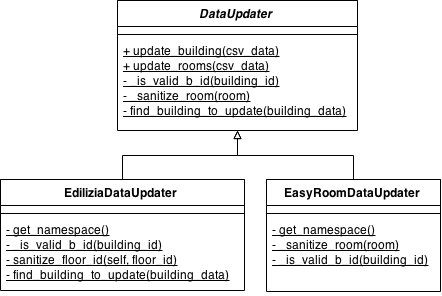
\includegraphics[width=280pt,natwidth=442,natheight=296]{class_diagram_dataupdater_before.png}
    \caption{Si noti che in Python non sussistono veri vincoli di protezione
    sui livelli di accesso. Metodi privati sono indicati semplicemente con
    un underscore all'inizio, e rappresentano una convenzione.}
    \label{fig:class_diagram_dataupdater_before}
\end{figure}

Alla stesura della ``frase di responsabilità'' per DataUpdater, ho
ottenuto il seguente: 
``Gestire la validazione e aggiornamento dei dati delle stanze 
e/o palazzi in database e far partire la procedura di integrazione
con le altre sorgenti''. 
Dalla lunghezza della frase e della classe stessa e dalla quantità di 
congiunzioni, ho concluso che si trattava di una classe le cui responsabilità
era necessario spartire. Si trattava di una classe considerevolmente lunga, 
e sicuramente gestiva almeno due responsabilità distinte.

Approfittando dell'ereditarietà multipla fornita da Python, la separazione più netta
era stata quella di dividere DataUpdater in due classi, 
BuildingDataUpdater e RoomDataUpdater, facendo si che EdiliziaDataUpdater 
e EasyRoomDataUpdater ereditassero da entrambe. Un altra possibilità 
sarebbe quella di favorire la composizione invece di usare l'ereditarietà\footnote{
\textit{Favor composition over inheritance} - un altro principio di
design del software.
}. 
Ho deciso per l'ereditarietà per due motivi: non avevamo richieste di 
cambiamenti a \textit{runtime}, e non esistevano metodi o attributi 
in comune utilizzati da BuildingDataUpdater e RoomDataUpdater, il che garantiva 
che non si sarebbe verificato nessun dei noti problemi di 
\textit{method resolution 
order} che nascono in contesti di ereditarietà multipla. Da questo cambiamento
siamo passati al seguente \textit{class diagram}:

\begin{figure}[H]
    \centering
    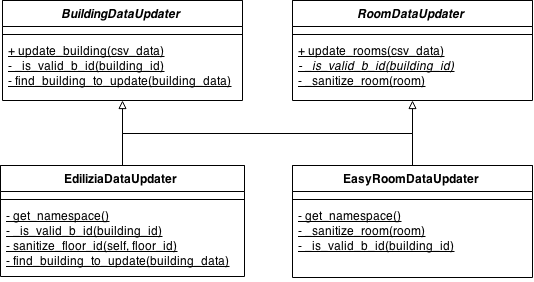
\includegraphics[width=340pt,natwidth=534,natheight=282]{class_diagram_dataupdater_after.png}
    \caption{La separazione di DataUpdater in due classi diverse. Si noti
    che i metodi delle sottoclassi sono esattamente gli stessi. L'unico metodo
    duplicato è \_is\_valid\_b\_id(building\_id), che è astratto
    su RoomDataUpdater. L'ho aggiunto al diagramma per correttezza 
    sintattica dato che viene chiamato dal metodo update\_rooms. La semantica
    richiesta del metodo è ovviamente la stessa in entrambe le classi.
    In Python, essendoci il \textit{duck typing}, non è mandatoria la
    dichiarazione di metodi astratti. 
    }
    \label{fig:class_diagram_dataupdater_after}
\end{figure}

Dopo aver sistemato i bug introdotti da questo cambiamento e rilevati 
correttamente dalla nostra suite di test, il risultato mi ha portato ad
ottenere due differenti frasi che descrivono le responsabilità:

\begin{itemize}
  \item RoomDataUpdater: ``Gestire la validazione e aggiornamento dei dati delle
  stanze in database e far partire la procedura di integrazione
con le altre sorgenti''
  \item BuildingDataUpdater: ``Gestire la validazione e aggiornamento dei dati 
  dei palazzi in database e far partire la procedura di integrazione
con le altre sorgenti''
\end{itemize}

Le frasi continuavano ad essere piuttosto corpose, ma adesso la responsabilità 
era stata divisa esattamente a metà. Una classe gestiva una tipologia di 
dati, un altra classe l'altra. Ma non ero soddisfatto. 

Avevo indossato il mio ``cappello del refactoring''\footnote{
Allusione alla metafora di ``Two Hats'' di Kent Beck, raccontata
da Martin Fowler in \cite{fowler2002}, in cui afferma l'importanza di
essere sempre cosciente di quale cappello stiamo utilizzando, ovvero 
di avere chiara la separazione tra il momento di implementare nuove 
funzionalità e quello di fare \textit{refactoring}.
}, e non volevo toglierlo (mi stava bene :D). 
Ho incominciato con RoomDataUpdater,
e ho provato ulteriori suddivisioni, cercando dei pattern 
da applicare e sono riuscito a fare un paio di modifiche. Alla fine di questa
serie di modifiche avevo raggiunto qualcosa che mi sembrava più ``modulare''.
Metto la parola modulare tra virgolette perché quello che avevo fatto in realtà
era stato frammentare quel flusso di esecuzione in una quantità elevata di
piccole classi che incapsulavano poca o nessuna unità logica di 
esecuzione. Il flusso dell'algoritmo era stato spezzato in modo che la sua
comprensione era praticamente impossibile.

La mia fortuna è che si trattava di fine giornata quando avevo dichiarato 
``compiuta'' quell'impresa. Ero stanco e dovevo ancora risistemare un paio
di test di unità che fallivano in conseguenza di quel refactoring perché
testavano l'esecuzione precedente in modo vincolato all'implementazione, e
allora ho deciso di lasciare la conferma (\textit{commit}) 
di quelle modifiche verso il nostro sistema di \textit{versioning}
per il giorno dopo.
La mattina successiva, ansioso per il primo \textit{commit} del giorno,
ho sentito di nuovo che ciò che avevamo fatto non era convincente,
ma non capivo il motivo.


Mi sono messo a rivisitare altri concetti di Progettazione 
Software, cercando qualcosa che mi
aiutasse a capire perché, dopo aver applicato così sistematicamente l'SRP
avevo un ulteriore impressione che ci fosse qualcosa di sbagliato.

\section{La Redenzione Attraverso il Concetto di \textit{Cohesion}}
Un po' per caso sono arrivato a rileggere informazioni
sul concetto di \textit{Cohesion}\footnote{
La coesione è una misura di 
quanto strettamente correlate siano le varie funzionalità messe a disposizione 
da un singolo modulo (o classe). Si intende come una buona qualità in 
software quando un modulo o classe è considerato coeso. Da non confondere
con il termine \textit{coupling}, che sta ad indicare un accoppiamento non 
necessario fra moduli/classi diversi e che genera più dipendenze e difficoltà
per il cambiamento, e di solito è considerato come un aspetto negativo.
}.
Nel tentativo di applicare il principio della \textit{singola} responsabilità
in modo praticamente fanatico, avevo violato la coesione logica e anche
temporale dell'algoritmo di partenza. Il motivo per cui il metodo update\_rooms
incapsulava quella sequenza di passi era funzionale, logico. Per inserire 
una stanza la dovevo prima pulire (formattando meglio le stringhe, ad esempio)
e validare (non dovevo inserire stanze che non godessero, ad esempio, di un
identificativo del palazzo a cui appartenevano). In seguito avrei preparato il
formato verso il database, inviato i dati e, una volta che i dati originali
di questa sorgente sarebbero stati memorizzati \textbf{correttamente}, 
avrei dovuto 
fare una richiesta a un'altra classe che avrebbe eseguito 
l'integrazione con altre sorgenti dati già presenti. 

Il compito funzionale delle mie classi sotto analisi era di gestire il 
flusso degli aggiornamenti, la catena di passi necessari.
Erano classi in cui gli elementi godevano di coesione di tipo:

\begin{itemize}
  \item Funzionale, perché miravano a risolvere uno stesso problema.
  \item Sequenziale perché ogni \textit{step} dipendeva del successo e usava 
  l'output di quello precedente.
  \item Di comunicazione perché lavoravano sugli stessi dati.
  \item Procedurale e temporale perché dovevano essere eseguiti in un preciso
ordine.
\end{itemize}

In altre parole, era giusto che tutto ciò fosse localizzato, in modo coeso, 
all'interno della stessa classe. Ancora una volta mi è rimasto evidente
quanto sia importante analizzare ogni caso
in modalità ad hoc, cercando di ottenere un equilibrio instabile tra concetti
diversi che, applicati ingenuamente arrivano pure a contraddirsi.
Non ci sono regole d'oro o operazioni che portino necessariamente
a un buon \textit{design}, per questo, infatti, parliamo di principi
e concetti invece di ``regole'', o \textit{code smells} invece di errori.

Ho concluso allora che il criterio suggerito da Sandi Metz 
per capire se ci sono più responsabilità in una stessa classe era
un po' estremo, e che più spesso conviene analizzare caso a caso. La
strategia di sintetizzare le responsabilità in una unica frase
è comunque utile nel renderle evidenti.

Avevo allora giustificato l'unione di quelle componenti all'interno della
stessa classe per il principio della coesione.
Ma non ero ancora soddisfatto. C'era qualcosa che, ancora, non andava bene!

\section{L'SRP con granularità diversa}

La definizione del Single \textit{Responsibilty Principle} più accettata
parla esplicitamente di classe. Più precisamente è definita nei seguenti 
termini: ``Una classe deve avere al massimo una ragione per cambiare''\cite{bobmartin2003}
\textit{
(Traduzione mia, originale in inglese\footnote{
  ``A class should have only one reason to change''
}).
}

Avendo capito meglio e anche nella pratica cosa effettivamente 
quest'affermazione significa, ho provato ad estendere la sua applicazione
non solo con granularità di classe, ma anche a livello di singolo 
metodo/algoritmo.

Una volta che il file CSV con le informazioni testuali dei palazzi
veniva letto, alla classe BuildingDataUpdater 
veniva delegato il lavoro di eseguire veramente l'aggiornamento, con 
la chiamata del metodo statico update\_buildings, che riceveva appunto la 
lista di informazioni da processare e finalmente inserire nel database. 
Come detto in precedenza, l'algoritmo sintetizzato prevedeva tutto il 
flusso per l'aggiornamento: validazione, pulizia e richiesta dell'integrazione
dei dati con le altre sorgenti già presenti in database (ad esempio le piante 
architettoniche). Tale algoritmo funzionava bene e godeva di una buona quantità
di test di unità e di accettazione. 

Il codice era funzionante ma era lungo e difficile da capire, e lo stesso
capitava anche per il metodo update\_rooms su RoomDataUpdater.
Dovevano gestire più aspetti ad ogni singolo \textit{step}:
validare (e eventualmente segnalare all'utente inconsistenze), formattare i
dati, memorizzarli, richiedere l'integrazione.

Analizzando la struttura di questi metodi e chiedendomi delle loro
responsabilità, ho concluso che la causa del \textit{code smell} non
era effettivamente a livello di classe ma del metodo stesso. 
Mancavano basiche applicazioni dei principi di \textit{Object Orientation},
estrazione di codici duplicati in metodi dedicati e una convenzione
di \textit{naming} delle variabili che ne favorisse la comprensione
del codice.

Avevo deciso allora di metterli a posto, ma non volevo rischiare di
ripetere l'errore precedente di frammentarli troppo. Per questo motivo, e
anche per il fatto che si trattavano di implementazioni molto fragili,
caratterizzate dalla costruzione di molti stati intermedi temporanei e
da una logica molto procedurale, ho deciso di eseguire questa
operazione di \textit{refactoring} a piccoli passi, appoggiandomi sui
test che avevamo già scritto per garantire che le modifiche riportate
non danneggiassero il comportamento originale del metodo.

\section{Gli effetti dell'applicazione sistematica dell'SRP}

Volevo evitare di innescare grossi contenuti di codice, ma sembra opportuno
inserire la versione originale e la versione finale del metodo update\_buildings
per illustrare la differenza. Si noti che per questo discorso non è necessario
capire il funzionamento o la logica della versione originale, ma più che
altro compararne la leggibilità (e dimensione!) rispetto alla versione ripulita. 
Per brevità ho accorciato le stringhe di stampa, 
dato che sono spesso messaggi lunghi e pieni di dettagli utili all'utente 
finale, e per chiarezza ho aggiunto commenti (non tutti presenti nell'originale) 
riga per riga.

\newgeometry{left=3cm, right=2.5cm}
\newpage
\pythonexternal[caption=Versione iniziale del metodo update\_buildings,frame=tlrb]{code_samples/building_data_updater_before.py}
\newpage
\restoregeometry

Non ci vuole molto per capire quanti problemi sussistono nel 
codice sopra, e per questo motivo evito di commentarlo e passo 
subito alla visione della versione finale, che esplicita i
problemi a partire dalla loro risoluzione:

\pythonexternal[caption=Versione finale del metodo update\_buildings,frame=tlrb]{code_samples/building_data_updater_after.py}
  
Da notare le seguenti proprietà di questo \textit{refactoring}:

\begin{itemize}
  \item Il metodo update\_buildings compie ora il ruolo
  di scheletro dell'esecuzione. Essendo piccolo, ci sta in una sola
  pagina di codice e permette con un unico sguardo di cogliere il flusso.
  \item L'esplicitare lo scheletro aiuta nel trovare
   eventuali problemi concettuali che dipendono dall'ordine
   delle operazioni.
  \item Ogni \textit{step} coincide con una chiamata di metodo, 
  che viene incapsulato e isolato. Cambiamenti della logica di
  lavoro, come ad esempio quella di validazione dei dati in input,
  da ora in poi avvengono in modo isolato, riducendo
  sostanzialmente il costo delle modifiche.
  \item Limita la profondità dell'indentazione (significativa in Python) 
  che rendeva la comprensione del metodo più difficile, e ci spingeva spesso
  ad abbreviare variabili con lo scopo di contenere la lunghezza massima
  delle righe. 
  È buona pratica in diversi contesti di programmazione 
  la manutenzione della lunghezza massima delle righe di codice su 
  80 caratteri\footnote{
  A titolo di curiosità, si suppone che questa convenzione sia stata 
  influenzata dai \textit{punchcards} IBM che inizialmente avevano 80 colonne.
  }, 
  per aumentare la leggibilità e far si che sia possibile visualizzare
  contemporaneamente due file diversi dividendo uno schermo standard
  in verticale. È particolarmente utile per l'attività di \textit{testing} 
  dato che la visione simultanea del test e del relativo codice testato
  rende più esplicita la loro relazione.  
\end{itemize}

Questi sono aspetti più correlati alla struttura del codice. Sono essenziali
specialmente per garantire l'incapsulamento delle unità funzionali, rendendole
meno dipendenti. In altre parole, favoriscono il disaccoppiamento tra i diversi
passi della logica del dominio applicativo. Questo incapsulamento all'interno
di metodi piccoli è particolarmente importante per i seguenti aspetti:

\begin{itemize}
  \item Metodi più piccoli sono, in linea di principio, più facili 
  da capire e allora è più probabile 
  che eventuali errori emergano in fase di lettura di codice,
  e che l'attività di \textit{debugging} diventi anche più semplice.
  \item Aumenta la \textit{testability} dell'algoritmo complessivo, in quanto
  ci fornisce un ulteriore strategia per il \textit{testing}: 
  per verificare la correttezza del metodo principale 
  possiamo procedere in modalità \textit{divide and conquer}, 
  testando i singoli \textit{metodi} (\textit{divide}) 
  che lo compongono, e poi verificando che le
  chiamate interagiscano nel modo corretto (\textit{conquer}).
  \item Essendo più piccoli, possono lavorare su un sottoinsieme 
  di informazioni e richiedere allora meno \textit{setup} 
  di strutture dati e contesti per l'esecuzione dei test. Di conseguenza
  su ogni singolo metodo, a parità di tempo e sforzo, vengono testati
  più casi e aspetti.
\end{itemize}

\section{Il codice ``auto-documentante''}

Per ottenere il risultato sopra sono partito con l'estrazione di unità 
funzionali in metodi dedicati, nominandoli nel modo che mi sembrava 
più opportuno al momento. Una volta concluse le estrazioni, però, guardando il
corpo del metodo principale, mi sono accorto che si poteva migliorare
la scelta dei suddetti nomi.

Durante la fase di studio e 
rielaborazione di questo codice, ho trovato un'idea interessante 
su cui mi sono basato, espressa da Kent Beck\footnote{
In una partecipazione nel libro \textit{Refactoring: Improving the 
Design of Existing Code} di Martin Fowler\cite{fowler2002}}, che 
mi ha guidato: 

\begin{quote}
	La scelta del nome di ogni classe e del nome di ogni metodo ci fornisce
	un'opportunità per spiegare quale sia la sua intenzione. Il corpo di
	ogni classe o metodo spiega a sua volta come quell'intenzione è stata
	realizzata. Se il corpo è anche scritto in termini di intenzione in
	pezzi ancora più piccoli, si può scrivere del codice che comunichi
	la maggior parte dell'importante informazione sulla sua propria struttura.
	- Kent Beck in \cite{fowler2002}.
	
	\flushright
	\textit{(Traduzione mia, originale in inglese\footnote{
			``Choosing the name of each class and the name of each method gives 
			you an opportunity to explain what you intend. The internals of the 
			class or method explain how the intention is realized. If the 
			internals also are written in terms of intention in yet smaller 
			pieces, you can write code that communicates most of the important 
			information about its own structure''
		})
	}
\end{quote}

In altre parole, una scelta non solo opportuna ma intelligente del nome delle
variabili, metodi e classi porta, oltre al vantaggio ovvio della leggibilità
del codice, a un codice ``auto-documentante''. È il codice stesso ad esprimere
il suo scopo, senza necessità di ausili esterni, ne di commenti, ne di documenti
formali. Gli effetti della scrittura di codice con queste qualità sono molti, 
e a noi interessava particolarmente il fatto di rendere più facile l'adozione
della \textit{codebase} in futuro per la continuazione del progetto.

In particolare nel caso di questo refactoring, i nomi più significativi
illustrano bene il flusso funzionale e la logica applicativa incorporata.
Inoltre, il rinominare della variabile di iterazione ``b'' a ``b\_data'' rende
più chiaro il suo scopo (sono i dati letti da inviare al database) 
e la differenzia dalla variabile building (che è un oggetto della
classe Building, un ODM\footnote{\textit{Object-Document Mapper}} Model che
rappresenta i documenti in database da aggiornare/inserire. 

È ovvio che la naturale espressività di un linguaggio come Python rende
più semplice il raggiungimento di queste caratteristiche. 

Le righe 4 e 5 comunicano che i dati dei palazzi verranno validati, 
e che quelli invalidi verranno semplicemente ignorati (\textit{continue}). 
Se sono interessato a capire qual'è la logica di validazione, mi basta
proseguire al metodo \_validate\_building\_data, definito 
sulla stessa classe. Si noti che si potrebbe portare ancora avanti 
la leggibilità, sfruttando la struttura di controllo fornita da Python 
per formare vere e proprie frasi in linguaggio naturale, con la 
rinominazione del metodo di validazione:

\begin{python}
if not self._is_valid_building_data(b_data):
    continue
\end{python}

È sicuramente più bello da leggere, ma la facilità di comprensione è la stessa,
e allora mi è sembrato un cambiamento opzionale. La decisione di dove fermarsi
va presa tenendo in considerazione il livello di espressività desiderato
e il tempo dedicato al refactoring. Senza imporci un limite preciso rischiamo
di stare troppo tempo ad eseguire piccoli cambiamenti che contribuiscono
di poco. La ricerca della perfezione va contestualizzata, altrimenti diventa
dannosa.

Esiste un ultimo aspetto che vorrei sottolineare sulla scelta intelligente
dei nomi, che ha reso esplicita la relazione fra le chiamate 
di metodo delle righe 8 e 13. Per garantire che ogni aggiornamento di
file CSV rappresentasse uno \textit{snapshot}, ovvero che se un giorno un
palazzo venisse rimosso dal ``catalogo''\footnote{
Può sembrare strano che un palazzo venga rimosso, ma ce ne sono casi in cui
succede, come ad esempio palazzi che non sono di proprietà dell'università
ma vengono rintracciati e allora possono in futuro non più venir utilizzati. 
Dovevamo inoltre gestire eventuali errori, come ad esempio inserimenti duplicati
con codici identificativi sbagliati, casi in cui bisogna rimuovere il duplicato
o sbagliato.
}
verrebbe cancellato anche dal nostro database, avevamo pensato a un algoritmo
che procedeva in modalità \textit{mark and sweep}: prima marcavamo tutti i palazzi
che erano stati contemplati in questo \textit{snapshot}, e, una volta
finiti gli aggiornamenti di tutti i palazzi, cancellavamo quelli
che non erano stati marcati. Si tratta allora di un algoritmo a due passi,
in cui il primo va fatto all'interno del ciclo \textit{for} di
aggiornamento, e il 
secondo alla fine. L'estrazione di questi \textit{step} in metodi dedicati
rende anche questa correlazione esplicita dal nome conferito ai metodi:
\_mark\_building\_as\_updated e \_destroy\_unmarked\_buildings.


\section{Conclusioni pratiche}

Come abbiamo visto, l'estrazione delle unità funzionali in metodi dedicati
favorisce l'applicazione di ulteriori refactoring in quanto ne limita 
l'impatto attraverso l'incapsulamento delle modifiche.
L'applicazione ripetuta e incrementale di operazioni di refactoring
ha reso i singoli metodi significativamente più piccoli e
semplici, rendendoli più mantenibili, disaccoppiati e testabili.

I metodi estratti sono talmente semplici che mi permetto di omettere 
il loro codice sorgente, dato che non contribuiscono al ragionamento 
fino a qui elaborato.

Ho finito l'attività di \textit{refactoring} di BuildingDataUpdater,
applicando altri principi sui singoli metodi, cercando più che altro
una buona leggibilità del codice,
e ho proceduto a un refactoring molto simile su RoomDataUpdater. 

Aver applicato l'SRP più volte su più livelli, e avendo potuto poi 
contrastarlo con in concetto di \textit{cohesion}, mi ha permesso 
di cogliere una significativa intuizione pratica da riapplicare in 
altri contesti, e la dinamica SRP / \textit{Cohesion} mi ha in seguito 
aiutato a riportare ulteriori \textit{refactoring} di tipo strutturale 
su altre classi, senza però compiere l'errore commesso nella 
prima applicazione.


%
%
%
%
\chapter{Refactoring continuo e guidato}
\label{cap:refactoring_continuo}

Analizzando queste esperienze, ho concluso che l'aver utilizzato uno o più
concetti esplicitamente per l'analisi del codice mi ha permesso di
cambiare l'approccio, lo sguardo, e mi ha reso capace di eseguire
modifiche più significative.

Da ciò segue l'importanza di avere un approccio sistematico al 
\textit{refactoring}, e che studiare le sue modalità e casi di applicazione
è una forte componente dell'esperienza di uno sviluppatore. Inoltre, partendo
dal \textit{refactoring} sentivo che le mie capacità di \textit{design}
miglioravano. Ad ogni classe rielaborata mi sentivo leggermente più
capace di sentire i \textit{code smells} ma anche di capire 
che cosa li generava.

Essendomi particolarmente interessato all'argomento, ho trovato un libro 
che mi ha cambiato il modo di vedere il problema già dalla prefazione.

Si trattava del libro ``Refactoring: Improving the Design of
Existing Code''\cite{fowler2002}, di Martin Fowler, sviluppatore, 
autore e \textit{public speaker} per cui provo una sincera ammirazione,
specialmente per il suo modo teorico-pratico di affrontare il nostro
mestiere. 

Già alla \textit{Foreword} scritta da Erich Gamma\footnote{
Erich Gamma (nato nel 1961 a Zurigo) è un ingegnere del software e
coautore dell'influente libro di Software Engineering ``Design Patterns: 
Elements of Reusable Object-Oriented Software'' e ha dato numerosi contributi
teorici e pratici (ad esempio ha creato il framework per il testing 
JUnit insieme a Kent Beck) sull'argomento.
}
sentivo di aver trovato un punto di riferimento, e mi sono stupito di
vedere che molte delle conclusioni a cui ero arrivato dopo
duri processi di tentativi, errori e riflessioni, venivano formalizzate
e trattate in modo chiaro ed esplicito.

Ho trovato una definizione più precisa di refactoring, e, più importante, 
ricorrenti incentivi alla sua 
\textbf{pratica continua}, a prescindere degli ostacoli naturali (management, 
l'impressione che non porti a niente di nuovo, molto sforzo per nessun valore
percepibile dall'esterno, eccetera). Un'idea su cui avevo appena riflettuto
ma che Martin Fowler ha molto bene sintetizzato è quella descritta nel
seguente paragrafo:

\begin{quote}
Senza il refactoring, il design del programma decade. A misura che le persone
cambiano il codice - modifiche per realizzare obiettivi immediati o modifiche
fatte senza una comprensione complessiva del design del codice - il codice
perde la sua struttura. Diventa più difficile capire il design leggendo
il codice. [...] La perdita di struttura del codice ha un effetto cumulativo.
Quanto più difficile è vedere il design del codice, più difficile è 
preservarlo, e più rapidamente esso decade. \textit{Refactoring} regolare aiuta
il codice a mantenere la sua forma. \cite{fowler2002} 

\flushright
\textit{(Traduzione mia, originale in inglese\footnote{
``Without 
refactoring, the design of the program will decay. As people change
code - changes to realize short-term goals or changes made without a full
comprehension of the design of the code - the code loses its structure. 
It become harder to understand the design by reading the code. [...] 
Loss of structure of code has a cumulative effect. The harder 
it is to see the design of the code, the harder it is to preserve 
it, and the more rapidly it decays. Regular refactoring helps 
code retain its shape.''
})
}
\end{quote}

Riflettendo su queste idee, mi sono accorto del
(primo) banale errore che avevo commesso, e mi 
sentivo ingenuo per quello: cercando sempre la ``buona progettazione'', 
abbiamo applicato principi e ragionamenti all'inserimento di nuove 
funzionalità, moduli e classi. Basandoci su estensiva sperimentazione, 
giudico che avevamo progettato bene ogni modulo / sistema 
prima della implementazione, e ci eravamo preoccupati 
di rielaborare ognuno di loro per un po' di tempo.

Però, anche se inizialmente concepiti con particolare cura della chiarezza, 
questi metodi venivano modificati con piccole correzioni e estensioni di 
comportamento. In questo naturale ciclo di vita di rielaborazione, 
trasformazioni, il design iniziale, complessivo, si perdeva, si appannava. 
Applicando l'attenzione per un buon design alle nuove funzionalità, ci 
siamo dimenticati di riadeguare quelle già esistenti!

Il secondo errore commesso è stato quello di frammentare eccessivamente la
classe BuildingDataUpdater durante il suo refactoring. Mi ero messo l'obbiettivo
di ``rimuovere una volta per tutte'' i \textit{code smells} su quella classe,
e allora mi sono messo a fare grossi cambiamenti. La verità è che l'unico
grosso cambiamento strutturale che era veramente necessario era quello di separare
DataUpdater in due classi distinte per l'aggiornamento delle stanze e dei 
palazzi, e poi eseguire operazioni più piccole di refactoring più localizzato:
la maggior parte erano estrazioni di metodi.

A rispetto della dimensione dei passi in fase di refactoring, Fowler, in
riferimento a un esempio presentato, è abbastanza chiaro:

\begin{quote}
La lezione più importante di questo esempio è il ritmo del refactoring:
testare, piccola modifica, testare, piccola modifica, testare. È questo
ritmo che permette al refactoring di procedere velocemente
e con sicurezza\cite{fowler2002}

\flushright\textit{(Traduzione mia, originale in inglese\footnote{
``The most important lesson from this example is the rhythm of refactoring:
test, small change, test, small change, test, small change. It is that
rhythm that allows refactoring to move quickly and safely''
})
}
\end{quote}

Quando parla di sicurezza, Fowler si riferisce all'importanza dei test,
nel garantire che le modifiche apportate non generino nuovi errori
su un codice che prima era funzionante. Da questa esperienza che vi ho
raccontato aggiungerei che il procedere a piccoli passi ci conferisce
anche un ulteriore livello di sicurezza: sulle modifiche nel design. 
A piccoli passi le trasformazioni avvengono in modo incrementale,
e allora esiste una maggiore probabilità di ridurre i tempi con cui 
riusciamo a percepire che il refactoring effettuato sia significativo 
e che ci stia portando nella direzione voluta.
Non posso dire che non avrei commesso quell'errore se fossi avanzato
a piccoli passi, ma di sicuro ci sarebbe una maggiore possibilità di non arrivare alla mattina per accorgermene.

Si noti inoltre il rilievo dato da Fowler all'idea di 
\textit{Refactoring Regolare}. Su questo aspetto si discute
ancora:

\begin{quote}
In quasi tutti i casi, mi oppongo all'idea di separare tempo da dedicare
al refactoring. Dal mio punto di vista refactoring non è un'attività a cui
si dedica un tempo preciso. Refactoring è qualcosa che si fa tutto il tempo
in piccole raffiche. Non si decide di fare il refactoring, ma se lo fa
perché si vuole fare qualcos'altro, e fare il refactoring ci aiuta a 
fare quella cosa\cite{fowler2002}.

\flushright
\textit{(Traduzione mia, originale in inglese\footnote{
``In almost all cases, I'm opposed to setting aside time for refactoring.
In my view refactoring is not an activity you set aside time to do.
Refactoring is something you do all the time in little bursts. You don't
decide to refactor, you refactor because you want to do something else,
and refactoring helps you do that other thing''
})
}
\end{quote}

Assumendo allora che questo approccio di \textbf{continuous refactoring} venga
portato avanti sin dall'inizio di un progetto, sono 
assolutamente d'accordo con tale affermazione. Con questo 
sforzo continuo e inerente all'attività di implementare nuove 
funzionalità o estendere quelle esistenti,
garantiamo che ad ogni passo il \textit{design} del codice non solo viene
mantenuto ma anche migliorato.

Nella mia opinione esiste però un caso in cui prendersi del tempo 
preciso per fare il refactoring è necessario. Si tratta del caso specifico che
ho sperimentato: quando ci si accorge un po' tardi che l'effetto 
cumulativo della perdita di struttura del codice ha già causato
troppi danni. A quel punto bisogna fermarsi, prendersi del tempo 
ed eseguire l'attività di refactoring a piena autonomia.

Vorrei sottolineare che c'è una netta differenza tra le due modalità
di refactoring. Nel primo caso (quando lo si esegue come
parte del processo di sviluppo stesso) utilizziamo il refactoring con lo
scopo di adeguare il codice esistente a delle richieste 
che dobbiamo implementare subito, e allora \textbf{richieste che conosciamo 
già}. Saranno appunto queste richieste a guidare 
i passi del refactoring: in che modo rielaborare il codice già esistente
per far si che l'aggiunta/estensione delle richieste funzionalità porti 
ad un design altrettanto elegante e talvolta anche migliore? 
Su questa tipologia di refactoring, Martin Fowler fornisce un lungo 
compendio di esempi pratici e di diverse
tecniche nel libro a cui faccio riferimento\cite{fowler2002}.

L'altro caso, cioè, quando decidiamo che lo stato attuale del codice
richiede un impegno dedicato di refactoring, non abbiamo richieste esplicite
a guidare le nostre trasformazioni. Le richieste invece tendono ad essere
piuttosto generali, come ``migliorare la leggibilità del codice'', ``ridurre
le dipendenze'', ``disaccoppiare moduli'', ``aumentare la testabilità'',
eccettera.

In questi casi diventa problematico, specialmente in visione di un
\textit{codebase} significativo, decidere da dove partire e scegliere
quali modifiche porteranno al maggior beneficio, dato che comunque
nei contesti pratici il tempo disponibile a un'attività del genere è 
anche limitato.

Nella mia particolare esperienza, i criteri utilizzati per guidare la scelta
di quali refactoring eseguire e su quali classi/moduli farlo, sono stati i
principi SOLID di cui ho prima parlato, con prevalenza dell'SRP. L'SRP è
stato il più utile perché molto spesso ho percepito che operare modifiche
sul codice in termini di riduzione delle responsabilità di ogni classe
rendeva più evidente problemi legati agli altri aspetti, come addirittura
il Liskov Substitution Principle. Definire bene le responsabilità di una classe
padre e delle sue classi figlio esplicitava la natura della relazione che
doveva sussistere fra di loro, e, di conseguenza, quali logiche funzionali
violavano l'LSP. 

Nel mio caso sento che questa strategia abbia funzionato bene, aiutandomi
nella scelta delle modifiche da operare e bilanciando in parte la
difficoltà di capire i problemi di design dovuta alla mancanza di un'esperienza
più SOLIDa (non per caso in maiuscole).


%
%
% 
%
%
\chapter{Il refactoring come attività di \textit{design}}
\label{cap:refactoring_come_design}

In ambito lavorativo, le scadenze e la pressione degli \textit{stakeholders}
fanno sì che molto spesso diventi difficile la manutenzione 
della qualità del software durante tutto lo sviluppo, 
a meno ovviamente di una forte resistenza da parte degli sviluppatori 
coinvolti, il che rischia addirittura di danneggiare
i rapporti professionali. È allora più naturale che in questo contesto la
preoccupazione riguardo al design e alla qualità del codice decada 
all'avvicinarsi delle scadenze, esperienza che anch'io ho vissuto più volte.

Su questo progetto sono partito 
con il preciso scopo di curare attentamente il \textit{design}. Ero
deciso a contenere la complessità della nostra \textit{codebase}
fin dall'inizio, per non ricadere ancora una volta in quella
situazione. 

Il concetto di \textit{design upfront} descrive l'attività di 
progettazione del software fatta a priori alla scrittura del codice 
stesso. Se da un lato è un'attività adeguata per determinate
tipologie di progetti, come nei rari casi in cui sono fissati e noti tutti i
requisiti in fase iniziale del progetto, dall'altro lato viene spesso criticata
per presupporre che gli sviluppatori abbiano la capacità di comprendere
tutti gli aspetti problematici senza un'estensiva attività di esplorazione. 
Viene particolarmente criticata negli ambiti di sviluppo \textit{agile} 
per non prevedere l'adeguazione ai cambiamenti: molte delle assunzioni
fatte in fase di progettazione si dimostreranno false, quando saranno già
state incorporate al \textit{design} o addirittura implementate. 

\section{Il paradosso dello sviluppatore}

Nel corso del progetto Spazi Unimi gli effetti della sistematica
rincorsa del design sono stati positivi in determinati ambiti, mentre 
su altri ci hanno generato moduli complessi e con eccessive indirettezze. 
Cercando di anticipare le richieste future, abbiamo predisposto strutture di 
base che poi non abbiamo effettivamente utilizzato. Abbiamo 
ottenuto più codice da mantenere, e una maggior difficoltà della 
comprensione dei flussi di esecuzione. 

Su questa problematica vorrei citare le riflessioni di Kent Beck
presentate in una sua partecipazione nel libro ``Refactoring: Improving the 
Design of Existing Code'' di Martin Fowler\cite{fowler2002}:


\begin{quote}
	
	Se si conclude il lavoro del giorno, ma se lo si fa in modo che diventi 
	impossibile la conclusione di quello di domani, allora siamo stati sconfitti.
	Da notare, però, che sappiamo cosa dobbiamo fare oggi, ma non siamo 
	sicuri sul domani. Forse faremo questo, forse quell'altro, o forse qualcosa
	che non abbiamo ancora nemmeno immaginato.
	
	\flushright
	\textit{(Kent Beck in \cite{fowler2002}, traduzione mia, originale in inglese\footnote{
			``If you get today's work done today, but you do it in such a way 
			that you can't possibly get tomorrow's work done tomorrow, then 
			you lose. Notice, though, that you know what you need to do today, 
			but you're not quite sure about tomorrow. Maybe you'll do this, 
			maybe that, maybe something you haven't imagined yet."
		})
	}
\end{quote}

Se da un lato Kent Beck avverte riguardo il rischio di implementare le 
funzionalità presenti in modo che quelle future diventino irraggiungibili,
dall'altro sottolinea che su quelle future non abbiamo nessuna certezza. 
A questa ambiguità do il nome di ``paradosso dello sviluppatore''.

Procedere nello sviluppo delle funzionalità pensando a ciò che dovremo
sviluppare in futuro comporta un \textit{overhead} che, con
grande probabilità, non verrà compensato: infatti, data la molteplicità
di cammini di sviluppo possibili, dobbiamo essere molto fortunati per
trovarne uno giusto.

L'incertezza è un ingrediente noto in ambito software, e nasce da diversi
aspetti, ad esempio dalla malleabilità del software che rende possibile
i frequenti cambiamenti dei requisiti. Se da un lato può essere semplice 
pianificare i lavori della prossima settimana, all'aumentare dell'orizzonte 
temporale l'effetto delle previsioni si degrada velocemente. Allo 
sviluppatore rimane da equilibrarsi tra le richieste di oggi e l'incertezza
del domani.

\section{Design \textit{a posteriori}: la tutela del \textit{refactoring}}

Riguardo a questa ambiguità, conseguenza della malleabilità del software, 
Kent Beck ci presenta una possibile via di uscita:

\begin{quote}
	Quando si percepisce che la decisione presa ieri non ha più senso oggi,
	si cambia quella decisione. Quindi si può fare il lavoro di oggi. Domani,
	alcune delle scelte di oggi sembreranno ingenue, e allora
	dovremo cambiare anche quelle.
	
	\flushright
	\textit{(Kent Beck in \cite{fowler2002}, traduzione mia, originale in inglese\footnote{
			``When you find that yesterday's decision doesn't make sense 
			today, you change the decision. Now you can do today's work. 
			Tomorrow, some of your understanding as of today will seem naive, 
			so you'll change that too.''
		})
	}
\end{quote}

Quando Kent Beck parla di cambiare le decisioni di ieri, non parla della
scelta delle funzionalità, ma dell'organizzazione
del codice e delle relazioni fra i moduli, cioè del design del software.
L'importanza è data non alla capacità di prevedere gli sviluppi futuri
del sistema, ma alla facilità con cui possiamo cambiare le decisioni
prese in passato, in modo da adeguare la soluzione esistente alle
nuove richieste appena arrivate. 

\begin{quote}
	Confrontate questo (il refactoring) con il dettagliato design
	a priori. Il design speculativo è un tentativo di includere
	tutte le caratteristiche positive nel sistema prima ancora che qualsiasi
	codice sia stato scritto. Il problema di questo procedimento è
	che è troppo facile prendere la decisione sbagliata. Con il refactoring,
	non si ha il rischio di essere completamente in errore. Alla fine
	il programma si comporta sempre come si comportava all'inizio.
	
	\flushright
	\textit{(Kent Beck in \cite{fowler2002}, traduzione mia, 
	originale in inglese\footnote{
			``Contrast this (refactoring) with careful upfront design. 
			Speculative design is an attempt to put all the good
			qualities into the system before any code is written. Then
			the code can just be hung on the sturdy skeleton. The problem
			with this process is that it is too easy to guess wrong.
			With refactoring, you are never in danger of being completely
			wrong. The program always behaves at the end as it did
			at the beginning. ''
		})
	}
\end{quote}

Questo è un approccio verticale rispetto alla
concezione tradizionale di design del software.
Si parla di refactoring, allora, come principio cardine del
design stesso. Non si tratta solo di correggere gli errori commessi, ma di
accogliere l'effimerità delle scelte attuali. Si tratta di sapere che, con grande
probabilità, domani esse verranno cambiate e che ciò è positivo per la
qualità del software. Facciamo il design a posteriori invece che a priori.

Questa coscienza ci porta a sviluppare le funzionalità di oggi nel modo
più semplice possibile, per limitare la quantità di codice scartato in futuro. 
Quanto più elaborate e complesse le scelte fatte oggi,
maggiore è, tendenzialmente, il loro sforzo implementativo. Se domani 
dovremo scoprire che parte del lavoro fatto non è più adeguato, ci conviene
piuttosto farlo nel modo più semplice possibile. 

Un concetto simile a questo descritto è il KISS, acronimo per l'espressione
\textit{Keep it simple stupid}, coniata nel 1960 da Kelly Johnson, ingegnere
aeronautico americano. Johnson affermava che gli aerei progettati 
dovevano essere riparabili facilmente da un qualsiasi meccanico,
con pochi e semplici strumenti. Questo concetto è stato ampiamente 
adottato nello sviluppo del software, e traduce esattamente 
questa rincorsa della semplicità.
Esiste anche una famosa frase sintetizzata da Brian W. Kernighan\footnote{
Computer scientist canadese, famoso, in particolare per i contributi allo
sviluppo di Unix e del linguaggio awk.}, che traduce
molto bene l'importanza della semplicità nella scrittura del codice: 
\textit{``
Debugging is twice as hard as writing the code in the first place. 
Therefore, if you write the code as cleverly as possible, you are, 
by definition, not smart enough to debug it.''}\footnote{
	Eliminare gli errori di un programma (``debuggare'') è due volte più
	difficile di scriverlo. Quindi, se scriviamo il codice nel modo più 
	intelligente che possiamo, non siamo, per definizione, sufficientemente 
	intelligenti per correggerlo.
}

Quindi, sviluppando per la semplicità, l'aggiunta di indirettezze 
o altri livelli di astrazione verrà 
svolta in seguito, quando effettivamente ne verificheremo la necessità. 
L'aggiunta di astrazione va fatta a partire dal refactoring, 
senza che porti dei cambiamenti sul comportamento del
sistema. Si basa allora su delle necessità reali, su un codice già
funzionante e su tutta la rete di protezione fornita dalla suite di 
test preventivamente definita. 

Come visto, ancora una volta lo sviluppo del progetto Spazi Unimi,
ci ha ricondotto al concetto di \textit{refactoring}: non più per sistemare
errori previamente commessi o rendere più leggibile il codice, 
ma per guidare, a posteriori, le trasformazioni sul design. 

Pensare al refactoring come attività di design, 
ci permette allora di circoscrivere la complessità del sistema alle 
astrazioni essenziali alla sua buona organizzazione. Queste sorgono 
da necessità concrete, a partire dal codice già esistente e funzionale.


\chapter{Conclusioni}

Partecipare a questo progetto mi ha presentato un'opportunità per
riflettere con calma sui principi della progettazione software, applicandoli
direttamente a un contesto pratico. 

Penso di aver colto aspetti importanti da considerare durante un 
\textit{refactoring} guidato, e allora di aver sanato alcune lacune e 
quella sensazione di ``mancanza'' e immobilità che avevo guardando i codici 
precedenti. Questo è stato possibile soltanto per il fatto che sono 
partito da riflessioni proprie, da uno sforzo lungo per capire i 
difetti di quel design, da tentativi pratici senza, appunto, 
la presenza di qualcuno che mi guidasse. In seguito a tanti tentativi
falliti o con successo soltanto parziale, e allora significativa riflessione
pratica, la letteratura e la teoria sull'argomento mi hanno aiutato a 
portare il ragionamento in avanti, a fare i salti di qualità
necessari.

La riflessione sulla letteratura mi ha anche aiutato a comprendere il 
motivo per cui inizialmente avevo sbagliato nei tentativi di refactoring,
frammentando troppo il flusso di esecuzione del codice 
in diversi moduli/classi, cioè la necessità
di procedere a piccoli passi, riflettendo su ogni
cambiamento compiuto e assicurandomi della correttezza con
l'esecuzione dell'insieme di test dedicati. 

Una volta che sono riuscito a compiere questi passi, ho cercato di riapplicare
il metodo utilizzando altri concetti. Mi rimane comunque la certezza che
mantenere un buon \textit{design} del software è un'abilità che viene acquisita
con esperienza, e con uno sforzo continuo. Non basta un ottimo design a
priori, perché questo viene fatalmente eroso man mano che riceve modifiche
e nuove funzionalità. Non basta neanche la voglia di mantenerlo, ci vuole
anche un \textit{know-how} la cui assimilazione non è direttamente 
proporzionale al tempo o allo sforzo impiegato, ma procede a salti irregolari.

Ciò che abbiamo fatto come team, in seguito a questi episodi, è stato appunto
dare dignità di processo all'attività di refactoring, inserendola all'interno
del nostro flusso di lavoro. Questo progetto è servito come applicazione 
pratica di tanti concetti che avevamo già studiato durante il nostro percorso
di studi, e, nel mio caso particolare, penso che ne abbia contribuito 
significativamente per farmi assorbire in modo più profondo alcuni dei
principi di Progettazione Software.

In letteratura ho trovato il riscontro che sentivo di aver bisogno per
poter sviluppare le mie proprie idee e capacità. Ciò rinforza in me l'idea
di aver scelto una professione in cui lo studio e l'aggiornamento costante 
sono fondamentali. Ma quello lo sapevamo già.

Concludo questo progetto con la sensazione che l'attività di design del software non sia affatto un'attività precisa, esatta. Ci vuole del tempo per maturare la propria comprensione del sistema in questione, il proprio sguardo e la percezione dei problemi. Ci vuole non solo contemplazione e riflessione, ma anche la possibilità di fare tentativi, commettere degli errori e confrontarsi. Questa esperienza ha contribuito alla formazione di una visione più matura, marcata dalla certezza che la strada da percorrere è ancora lunga e dal dubbio che ci sia una destinazione finale.
%

\nocite{*}
\printbibliography

% 
\end{document}
